\documentclass[useAMS,usenatbib]{mnras}
\usepackage[]{natbib,amsmath,amssymb,times,refname,bm}
\bibpunct{(}{)}{;}{a}{}{,}
%\linespread{1.0}
%\usepackage[utf8]{inputenc}
\usepackage{tabularx,amsmath,amssymb,hyperref}
\usepackage{graphicx,epsfig,color,latexsym}

\renewcommand{\d}{\mathrm{d}}
\newcommand{\e}{\mathrm{e}}
\newcommand{\ii}{\mathrm{i}}
\newcommand{\bea}{\begin{eqnarray}}
\newcommand{\eea}{\end{eqnarray}}
\newcommand{\be}{\begin{equation}}
\newcommand{\ee}{\end{equation}}
\newcommand{\rund}[1]{\left(#1\right)}
\newcommand{\vc}[1]{\mbox{\boldmath $#1$}}
\newcommand{\dc}{\partial}
\newcommand{\eck}[1]{\left[ #1 \right]}

\newcommand{\msun}{\,h^{-1}\,M_{\odot}}
\newcommand{\iobs}{I^{\rm obs}}
\defcitealias{Semboloni13}{S13}

\long\def\/*#1*/ {}

%\def\llabel#1{\label{sc:#1}  {#1}\hspace{0.5cm}}
%\def\elabel#1{\label{eq:#1}\fbox{#1}}
\def\llabel#1{\label{sc:#1}}
\def\elabel#1{\label{eq:#1}}

\sloppy

\title[Colour gradient bias]
{Calibration of colour gradient bias in shear measurement using CANDELS}
\author[Xer et al.]%
{
X. Er$^1$ \thanks{er.xinzhong@oa-roma.inaf.it},
H. Hoekstra$^2$, T. Schrabback$^3$, V. F. Cardone$^1$, R. Scaramella$^1$, R. Maoli$^4$,
\newauthor{M. Vicinanza$^{1,4,5}$, B. Gillis$^{6}$ L. Miller$^{7}$, J. Rhodes$^{8,9}$}
\\
$^1$ I.N.A.F. - Osservatorio Astronomico di Roma, via Frascati 33, 00040 - Monte Porzio Catone, Roma, Italy\\
$^2$Leiden Observatory, Leiden University, PO Box 9513, NL-230 RA, Leiden, the Netherlands \\
$^3$Argelander Instutite fuer Astronomie, Auf dem Huegel 71, D-53121 Bonn, Germany\\
$^4$Dipartimento di Fisica, Universita di Roma "La Sapienza", Piazzale Aldo Moro, 00185 - Roma, Italy\\
$^5$Dipartimento di Fisica, Universita di Roma "Tor Vergata", via della Ricerca Scientifica 1, 00133 - Roma, Italy\\
$^6$Royal Observatory, University of Edinburgh, Blackford Hill, Edinburgh EH9 3HJ, UK\\
$^7$Department of Physics, Oxford University, keble Road, Oxford OX I 3RH, UK\\
$^8$Jet Propulsion Laboratory, California Institute of Technology, 4800 Oak Grove Drive, Pasadena, CA 91109, USA\\
$^8$California Institute of Technology, 1200 East California Blvd, Pasadena, CA 91125, USA
%$$
}
\date{Accepted --;  received --;  in original from \today}
\pubyear{2016}

\begin{document}
\maketitle

\begin{abstract}
{\it Euclid} will image about two billion galaxies that can be used to infer cosmological
parameters using weak gravitational lensing. Exploiting the precision afforded by these
data relies critically on our ability to correct for instrumental effects, such as the convolution
by the point spread function (PSF). A complication is the fact  that the optical data
are obtained using a broad bandpass (550-920\,nm) while the diffraction-limited PSF depends
on wavelength. This leads to biases in the recovered galaxy shapes because the colours of 
galaxies vary spatially.  We show that the colour-gradient bias can be determined with high accuracy in simulated
noisy data. We also find that higher order image distortions, such as flexion, enhance
the bias, which may be relevant for the study of lensing in high density regions.
We estimate the size of this colour-gradient biases using multi-band observations 
from the {\it Hubble} Space Telescope and find correlations with the colours and sizes of
the galaxies, but do not observe a significant dependence with redshift. 
{\bf We need some concluding remark about the impact for Euclid.}

\end{abstract}
\begin{keywords} cosmology, weak lensing, systematics
\end{keywords}

%\vspace{1.0\baselineskip}

\section{Introduction}

The images of distant galaxies are distorted, or sheared, by the tidal effect of the gravitational  potential generated by intervening matter; an effect commonly referred to as weak gravitational lensing \citep[see e.g.][for a detailed introduction]{Bartelmann01}. The resulting correlations in the shapes can be related directly to the statistical properties of the mass distribution in the Universe, which in turn provide depend on cosmological parameters. Hence weak gravitational lensing by large-scale structure, or cosmic shear, has been identified as a powerful tool for cosmology. The measurement of the signal as a function of cosmological time is sensitive to the expansion history and the growth rate of large-scale structures, and thus can be used to constrain models for dark energy and modified gravity.

A useful measurement of the cosmic shear signal requires averaging over large numbers of galaxies
to reduce the uncertainty caused by the intrinsic ellipticities of galaxies. The result is, however, only meaningful if biases in the shape estimates are negligible. Various instrumental effects change the observed ellipticities by more than the typical lensing signal, which is of order one per cent. The most dominant source of bias is the smearing of the images by the point spread function (PSF), driving the desire for space-based observations \citep{Paulin-Henriksson08, Massey13}.
Despite these observational challenges, the most recent cosmic shear studies are starting to yield competitive constraints on cosmological parameters \citep{Heymans13, Jarvis16,Jee16,Hildebrandt17}. These results are based on surveys of modest areas of the sky, which limits their ability to study the nature of dark energy; to achieve that requires more than an order of magnitude improvement in precision.

Such a measurement is the objective of {\it Euclid} \citep{Laureijs11}, the dark energy mission of the European Space Agency (ESA) that will survey the 15\,000 deg$^2$ of extragalactic sky that have both low extinction and zodiacal light. To reduce the detrimental effects of noise on the shape measurements, the images used for the lensing analysis are observed using a wide bandpass (550-920\,nm). The much smaller PSF in space-based observations 
is a major advantage, but the diffraction-limited PSF leads to new complications. 

The most prominent one is that the correction for the smearing by the chromatic PSF depends on the spectral energy distribution (SED) of the galaxy of interest \citep{Cypriano10, Eriksen17} and ignoring this would lead to significant biases in the case of {\it Euclid}. Fortunately this can be accounted for using the supporting broad-band observations that are used to derive photometric redshifts for the sources: the correction employs an effective PSF which is derived from the estimate of the observed SED of the galaxy. This correction is sufficient if the SED does not vary spatially. If this is not the case, the underlying brightness distribution, which is needed for an unbiased estimate of the shear, cannot be unambiguously recovered from the observed images.
This results in a higher order systematic bias, which we call colour-gradient (hereafter CG) bias.
As shown by \cite{Semboloni13} (\citetalias{Semboloni13} in the rest of this paper) the amplitude depends on several factors: the SED of the galaxy, the relative size of the galaxy compared to the PSF, and the width of the bandpass, $\Delta\lambda$.  For instance, the bias scales as $\Delta\lambda^2$, and thus is particularly relevant in the case of {\it Euclid}.

Galaxies show a wide variety in colour gradients, with elliptical galaxies typically showing negative colour gradients (redder in the centre and bluer in the outskirts), with steeper gradients more commonly found in bluer or more luminous early type galaxies \citep[e.g.][]{2011MNRAS.414.3052D,
2011MNRAS.411.1151G}. Moreover, correlations between colour gradients and the overall colours and luminosities of the galaxies have been inferred \citep[e.g.][]{2010AJ....140.1528L, 2016A&A...593A..84K}.
Hence the relation between galaxy morphology and density may cause the CG bias to vary across the sky and may lead to correlations with the lensing signal itself. 

It is important that all systematic sources of biases are accounted for to a level that is smaller than the 
statistical uncertainties. In the case of {\it Euclid} this leads to tight requirements, as detailed in 
\cite{Massey13} and \cite{Cropper13}. Initial studies by \cite{Voigt12} and \citetalias{Semboloni13} used simulated images to show that the CG bias could be substantial,
exceeding nominal requirements for the multiplicative bias in the shear. They also argued
that it should be possible to calibrate the bias using {\it Hubble} Space Telescope (HST) observations
of a large sample of galaxies in the F606W and F814W filters. However, their conclusions are based on the analysis of simulated noiseless data. In this work, we revisit the issue of the calibration of CG bias,
with a particular focus on determining the bias from data with realistic noise levels. 

In Sect.~\ref{sec:concepts}, we describe the main concepts and introduce the notation. We present the results from the analysis of simulated images in Sect.~\ref{sec:simulations}. In particular we explore the  impact of having to use noisy data to measure the CG bias in Sect.~\ref{sec:noisy}.
In Sect.~\ref{sec:candels} we estimate the CG bias using HST observations from the Cosmic Assembly Near-infrared Deep Extragalactic Legacy Survey \citep[CANDELS;][]{Koekemoer11}.

%%%%%
\section{The origin of colour gradient bias}
\label{sec:concepts}

Following the notation of \citetalias{Semboloni13}, we consider an image of a galaxy, and denote the photon brightness
distribution of the image at each position $\bm \theta$ and wavelength $\lambda$ by $I({\bm \theta};\lambda)$, which is related to the intensity $S({\bm\theta};\lambda)$ by $I^0(\theta;\lambda)=\lambda S({\bm\theta};\lambda)
T(\lambda)$, where $T(\lambda)$ is the normalised transmission. We take this to be a top-hat with a
width $\Delta\lambda$ around a central wavelength $\lambda_{\rm cen}$. The resulting image of the galaxy, observed using a telescope with a PSF $P({\bm \theta};\lambda)$  is given by:
%
\be
I^{\rm obs}({\bm\theta}) = \int_{\Delta\lambda} I^0({\bm\theta}; \lambda) *  
P({\bm \theta},\lambda)\, \d \lambda,
\label{eq:iobs}
\ee
%
where $*$ denotes a convolution. 

A measurement of the ellipticity of a galaxy provides an unbiased (but noisy) estimate of the 
weak gravitational lensing signal, quantified by the complex shear $\gamma=\gamma_1+\ii\gamma_2$.
The ellipticity $\epsilon$ in turn can be determined from the second order brightness moments $Q^0_{ij}$ of the PSF-corrected image $I^0(\theta)$:
%
\be
\epsilon_1+\ii \epsilon_2 \approx \frac{Q^0_{11} - Q^0_{22} + 2 \ii Q^0_{12} }
{Q^0_{11} + Q^0_{22} +2(Q^0_{11}Q^0_{22} - (Q^0_{12})^2)^{1/2}}
\elabel{mshear}
\ee
%
where the second order brightness moments are given by\footnote{We implicitly assume that the moments are evaluated around the position where the dipole moments vanish.}
%
\be
Q^0_{ij} = {1 \over F} \int  I^{0}({\bm \theta})\, \theta_i \theta_j \, \d^2 {\bm \theta} \quad\; (i,j=1,2),
\ee
%
where $F=\int \d^2{{\bm\theta}}  I^{0}({\bm\theta})$ is the total observed photon flux.

In practice, however, the observed moments are measured from the PSF-convolved image given by
Eqn.~(\ref{eq:iobs}). Moreover, the moments are evaluated using a weight function $W({\bm\theta})$  to reduce the effect of noise in the images. Hence, the observed quadrupole moments are given by
\be
Q^{\rm obs}_{ij} = {1 \over F_{\rm w}} \int_{\Delta\lambda} \d\lambda \int \d^2 {\bm\theta} \,
I^0(\theta; \lambda) *  P(\theta,\lambda)\, \theta_i \theta_j \, W({\bm \theta})\,,
\ee
%
where $F_{\rm w}$ is the weighted flux. The use of a weight function biases the observed moments, 
and the aim of moment-based shape measurement algorithms is to correct for this using estimates of the higher order moments \citep[e.g.][]{Kaiser1995,Melchior11}. An alternative approach is to fit sheared, PSF-convolved models to the observed images 
\citep[e.g.][]{Bridle02,Miller13}; in these fitting methods the profile itself acts as a weight. 

\citetalias{Semboloni13} showed that the inevitable use of a weight function gives rise to the CG bias.
Consequently, the bias depends on the choice of the weight function, and vanishes in the case of {\it unweighted} moments. In the latter case it possible to determine the PSF-corrected moments $Q^0_{ij}$ from the observed quadrupole moments because
%
\be
Q^{\rm obs}_{ij}=Q^0_{ij}+P^{\rm eff}_{ij} \,
\ee
%
for unweighted moments, where $P^{\rm eff}_{ij}$ are the quadrupole moments of the effective PSF,  defined as
\be
P_{\rm eff}({\bm \theta}) = \frac{1}{F} \int \d \lambda\, P({\bm \theta},\lambda)\, F(\lambda) \,,
\ee
where   $F(\lambda)$ is the photon flux as a function of wavelength, which is directly related to the spectral energy distribution (SED) of the galaxy. Hence the correction for the chromatic PSF requires an estimate of the SED.  \cite{Eriksen17} have shown that the broadband observations that are used to determine photometric redshifts for {\it Euclid} can also be used to estimate the effective PSF with sufficient accuracy to meet the stringent requirements presented in \cite{Cropper13}.

%
\begin{figure*}
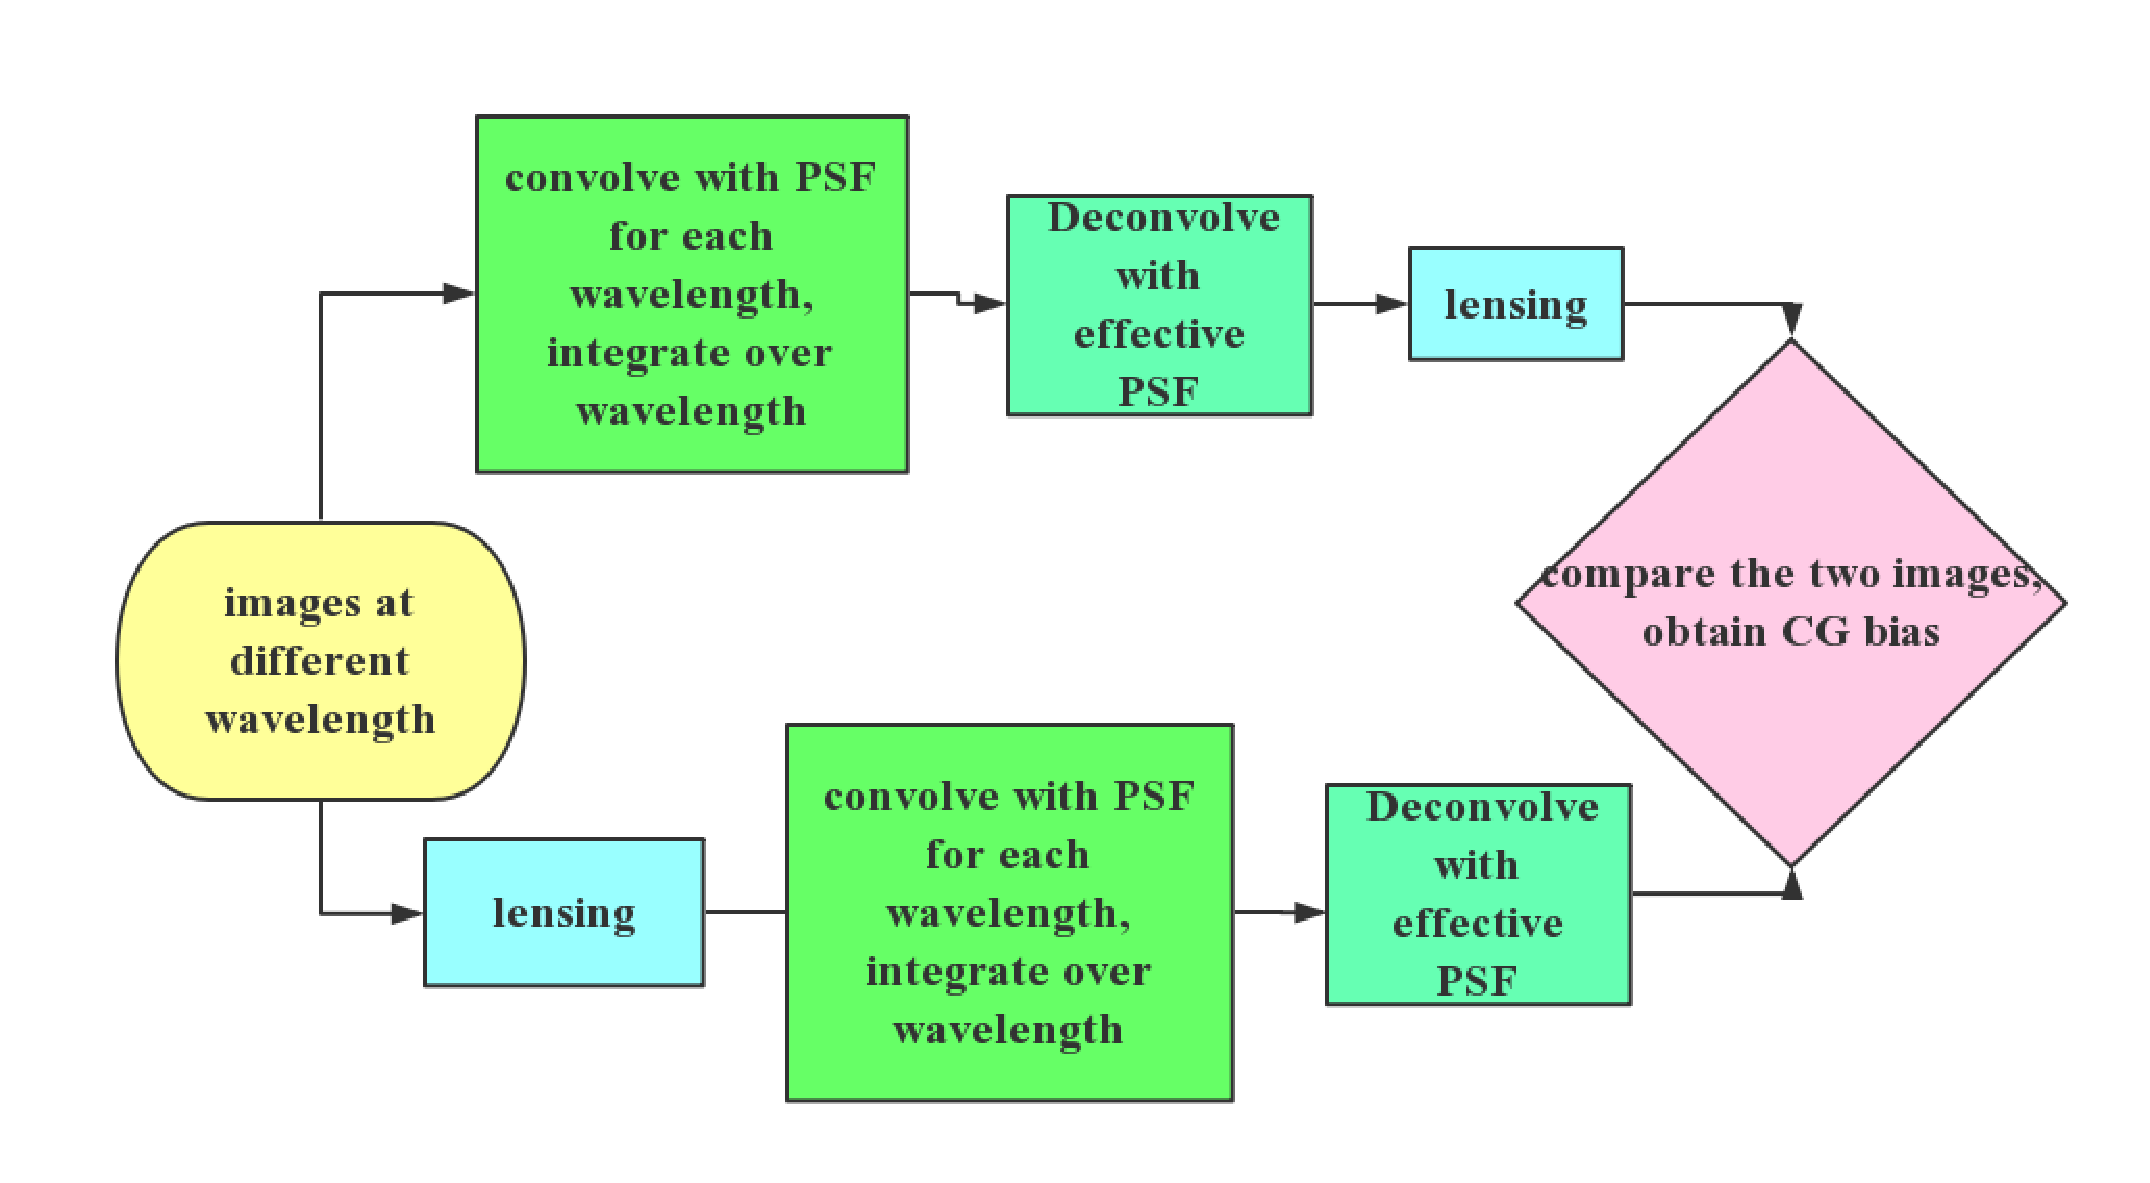
\includegraphics[width=12.5cm]{colourg.eps}
\caption{Flowchart describing how the colour-gradient bias is determined. The initial image
is the same in both flows, but in the top flow an image without a colour gradient is created
to which a shear is applied. In the bottom flow, the image is sheared before the PSF steps
are applied. The ellipticities of the resulting images differ slightly, and can be used to quantify
the bias that is introduced.}
\label{fig:flowchart}
\end{figure*}
%

We limit our study of the CG bias to the multiplicative bias it introduces, and our approach to quantify 
the impact on the lensing signal is similar to \citetalias{Semboloni13}. Figure~\ref{fig:flowchart} shows the flowchart of the steps that enable us to evaluate the CG bias.  In both cases we start with the same wavelength dependent image $I^0({\bm \theta};\lambda)$, but the bottom flow resembles what happens in the actual observations: the original image is sheared\footnote{We use 
$\gamma_1=0.05$  and $\gamma_2=0.02$ as reference, but we verified that other values yield similar results.} before the convolution with the PSF. The deconvolution with the effective PSF then yields the PSF-corrected shape. In the top flow the PSF steps are applied first, resulting in an image without a colour gradient that is subsequently sheared. 

We measure the ellipticities of the resulting images to estimate the CG bias. To reduce noise in our estimate of the multiplicative bias $m$ we use the ring-test method \citep{Nakajima07} where we create eight copies of the original galaxy but with different orientations. The ensemble averaged ellipticities then  provide an estimate of the multiplicative CG bias, $m$ (we do not explore additive bias here), via
%
\be
m= {\epsilon_i^{\rm CG} \over \epsilon_i^{\rm NCG} }-1,
\ee
%
where `CG' indicates the case where the galaxy has a colour gradient, and `NCG' is the galaxy
with a uniform colour. Note that our approach differs slightly from that in \citetalias{Semboloni13}, who quantify the response of the observed ellipticity to an applied shear. Hence, they do not apply the last step
in the bottom flow (the deconvolution), but rather convolve the final image in the top flow. 
The steps presented in Fig.~\ref{fig:flowchart} yield a more symmetric result, highlighting the fact
that the CG bias is the consequence of the fact that the shearing of the image does not commute 
with the convolution with the PSF. However, we verify in Sect.~\ref{sec:simulations} that we recover
the results of \citetalias{Semboloni13} (see Fig.~\ref{fig:biasofweight}). 

Recently, \cite{Huff17} proposed a technique to infer multiplicative shear calibration parameters that avoids the use of extensive image simulations, such as those described in \citep{Hoekstra17}. They quantify the 
sensitivity to a known shear by applying it to the observed data. Hence, their approach follows the top flow in Fig.~\ref{fig:flowchart} and thus cannot account for CG bias. 

\section{Colour gradient bias in simulated data}
\label{sec:simulations}

The CG bias is a higher order systematic bias, and thus the changes in the measured ellipticities are small. It is therefore important to verify that numerical errors in the calculations are subdominant compared to the small effects we aim to measure. To do so, we compare results from two independent codes that are used to generate the simulated images: one is written in C/C++ and the other uses the
python-based {\sc GalSim} package \citep{Rowe15}, which is widely used to created simulated images \citep[e.g.][]{FenechConti17, Hoekstra17}. 
  
In the C code we compute the image by multiplying the surface brightness at the centre of each pixel using a sheared S{\'e}rsic profile with the pixel area. In the case of {\sc GalSim} we use the {\sc Shear()} function (which convolves the image by the pixel). Since we are interested in small differences in the shapes of
deconvolved images, we first examined the size of potential numerical errors. We therefore convolved and
subsequently deconvolved elliptical images. Comparison of the recovered ellipticities revealed small differences between the codes that ranged from $10^{-7}$ to $10^{-6}$, two orders of magnitude
smaller than the CG biases we are concerned with. Hence can safely neglect this numerical artefacts here.

As a further test we compare directly to the results obtained by \citetalias{Semboloni13} for two reference galaxy models.  The reference galaxies are modeled as the sum of a bulge and disk component. To describe the wavelength dependence of the images we use the galaxy SED templates from \citet{1980ApJS...43..393C}: we use the SED for an elliptical galaxy for the bulge and take the SED of an irregular galaxy for the disk. This choice ensures that the resulting colour gradients are large. The two components are  described by a circular S{\'e}rsic profile:
\be
I_{\rm S}(\theta) = I_0 {\rm e}^{-\kappa\; \left(\frac{\theta}{a}\right)^{1/n}},
\ee
%
where $I_0$ is the central intensity, and $\kappa=1.9992\,n -0.3271$. For the bulge component we adopt $n=1.5$ and for the disk we use $n=1$. The profiles are normalised such that the bulge contains 25\% of the flux at a wavelength of 550\,nm. The galaxies are circular and the sizes for the bulge and disk for galaxy `B'   are $0\farcs17$ and $1\farcs2$, respectively. The second galaxy `S' is smaller with sizes of $0\farcs09$ and $0\farcs6$  for the bulge and disk, respectively (also see Table~3 in \citetalias{Semboloni13}). We create images with a size of  $256\times256$ pixels, and resolution $0.05$ arcsec/pixel at wavelengths 1\,nm apart and sum these in the range $550-920$\,nm to mimic the {\it Euclid} pass-band.

To create the PSF-convolved images we consider several PSF profiles. For a direct comparison with \citetalias{Semboloni13} we use their reference PSF1. As discussed in \citetalias{Semboloni13} this PSF has a similar size as the nominal {\it Euclid} PSF, but a steeper wavelength-dependence. Our implementation of the pipeline was able to reproduce the results presented in \citetalias{Semboloni13}.
To better approximate the {\it Euclid} PSF \citetalias{Semboloni13} also considered a model that  consists of a compact Gaussian core and an appropriately scaled top-hat (their PSF3). Instead we use here a more realistic obscured Airy profile, which is actually close to the {\it Euclid} design profile \citep{Laureijs11}:
%
\be
P(\theta) = {I_0 \over (1-\epsilon^2)^2} \rund{{2J_1(\theta)\over \theta} - 
{2\epsilon J_1(\epsilon \theta) \over \theta}}^2,
\elabel{psfairy}
\ee
%
where $I_0$ is the maximum intensity at the center, $\epsilon$ is the aperture obscuration ratio, and $J_1(x)$ is the first kind of Bessel function of order one; $x$ is defined as $x=\pi \theta/\lambda\, D $.
In the case of {\it Euclid}, $D=1.2$m and $\epsilon=1/3$. We compare this model to the Gaussian
case and PSF3 from \citetalias{Semboloni13} in Fig.~\ref{fig:psfmodel} at the 550\,nm and 920\,nm.

\begin{figure}
\centerline{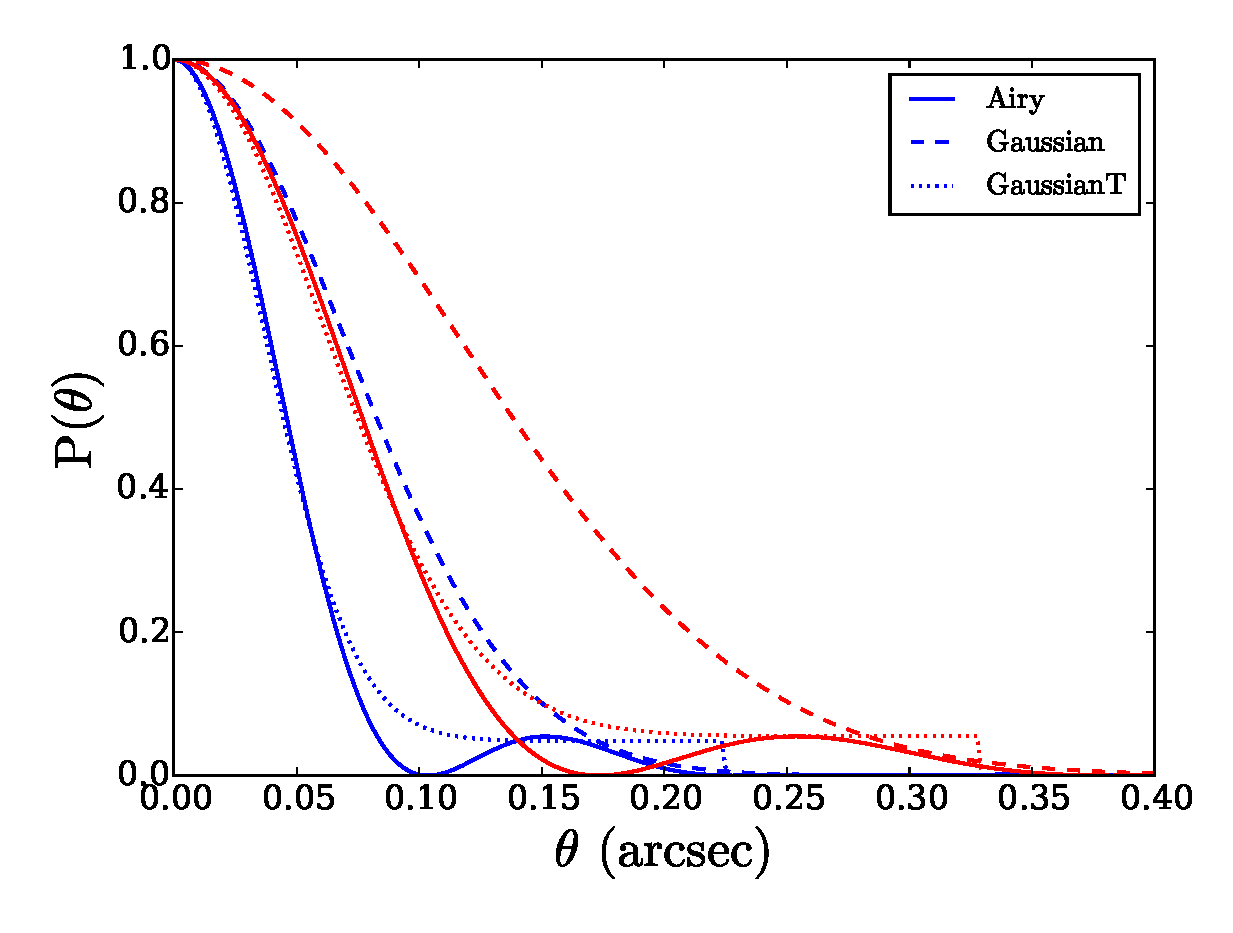
\includegraphics[width=\hsize]{zairy.eps}}
\caption{Comparison of the obscured Airy profile (solid), which is a good approximation
to the {\it Euclid} PSF, to PSF1 (Gaussian; dashed) and PSF3 (compact Gaussian and 
top-hat; dotted) from \citetalias{Semboloni13}. The profiles for 550\,nm are indicated by the blue lines and
the results for 920\,nm are shown in red.}
\label{fig:psfmodel}
\end{figure}
%

As discussed in Sect.~\ref{sec:concepts} the amplitude of the noise bias depends on the width of the weight function that is used to compute the (weighted) quadrupole moments. In Fig.~\ref{fig:biasofweight} we show the CG bias for the two reference galaxies as a function of $\theta_{\rm w}$, the width of the weight function that is used to compute the quadrupole moments. The results from the {\sc C} code (dashed lines) and the {\sc GalSim} code (dotted lines) agree very well for both the large galaxy `B' (red lines) and the small galaxy `S' (blue lines). Given the consistent results between the {\sc C} and {\sc GalSim} code we conclude that numerical errors are negligible in our implementation. In the remainder, we limit the simulations to those generated with {\tt GalSim}.

Figure~\ref{fig:biasofweight} shows that the CG bias decreases rapidly when the width of the weight function is increased. This allows for an interesting trade-off between CG bias and noise bias. The latter increases with increasing $\theta_{\rm w}$ but relatively slowly (see Fig.~4 in \citetalias{Semboloni13}). As a proxy for the optimal weight function (which maximizes the signal-to-noise ratio) we adopt the value of the 
half-light radius in the remainder of this paper. This yields $m=0.8\times10^{-3}$ for galaxy `B' and
$m=2\times10^{-3}$ for galaxy `S', demonstrating that the CG bias is a strong function of galaxy size.

%
\begin{figure}
  \centerline{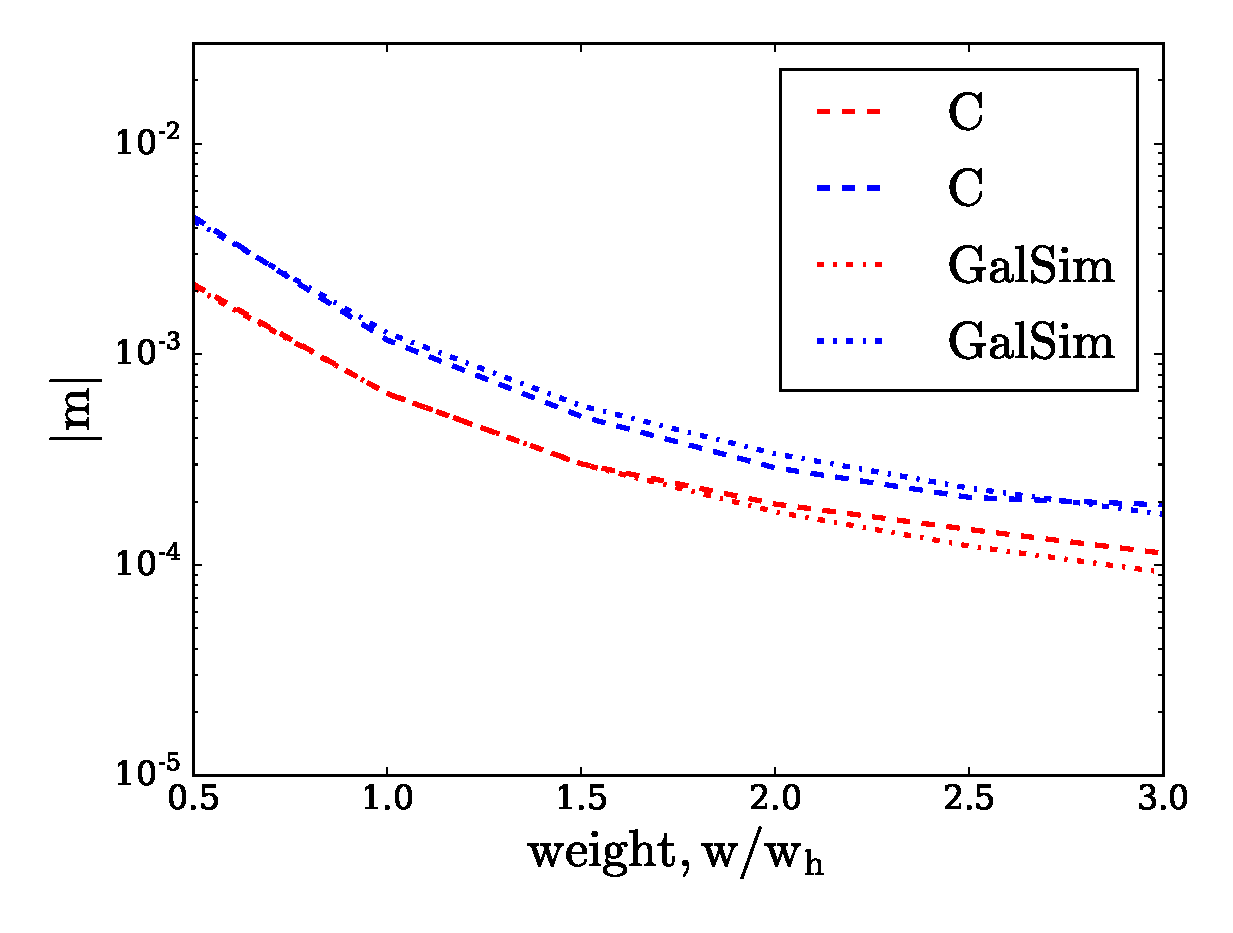
\includegraphics[width=\hsize]{zweight_airy.eps}}
\caption{The CG bias in shear versus width of the weight function (in
  units of the half-light radius $w_{\rm h}$) used to compute the
  quadrupole moments for the large (`B'; red) and small (`S';
  blue) reference galaxy. The galaxies were convolved using the obscured Airy
  PSF. The dashed (dash-dotted) lines are our
  results for images simulated using the {\sc C} ({\sc GalSim}) code.}
\label{fig:biasofweight}
\end{figure}
%
\subsection{Impact in high-density regions}

The focus of this paper is to quantify the impact of CG bias on cosmic shear measurements, 
i.e. we consider only small distortions in the shapes of the sources. However, {\it Euclid} will
also enable the calibration of the masses of galaxy clusters with unprecedented precision.
\cite{Koehlinger15} have shown that this should be possible given the accuracy required 
for the shape measurement algorithms for cosmic shear. This does implicitly assume that the 
performance does not change in high density environments. Blending does impact the performance
\citep{Hoekstra17}, but can be accounted for. In this section we focus instead on the unexplored question
whether the CG bias differs in the central regions of galaxy clusters.

In high density regions, higher order distortions of the images can become dominant. For instance, flexion (the next order after shearing) has been studied as a potential observational tool
\citep[e.g.][]{2002ApJ...564...65G,bacon2006}. Rather than simply shearing the images, as we have done so far, in this section we use the full lens equation to perform ray tracing simulations instead. This enables
us to capture the effect of the higher order distortion. For this exercise we use the {\sc C} code, as it has
this functionality fully implemented. As a lens we consider a singular isothermal sphere (SIS) with
an Einstein radius $\theta_{\rm E}=1$ arcsec. The image sizes are increased to $2048\times2048$ pixels, with a resolution $0.0125$ arcsec/pixel. 


{\bf we need to clarify what was exactly done; very interesting result so we need to explain this well.}

We move the lens from a large distance to the image and
calculate the CG bias at each distance. Fig.~\ref{fig:biasofgamma}
presents the bias with the tangential shear $\gamma_t$. The dotted
lines are the reference for the bias of sole shear, which agree with
the output of full lensing process (solid lines) when the shear is
small ($\gamma_t<0.1$). The difference becomes non-negligible if the
image is strongly lensed, and the full lensing process is necessary.
However, the typical cosmic shear is of order a few per cents. Hence
the large distortions will not cause significant effect in this work.


%
\begin{figure}
  \centerline{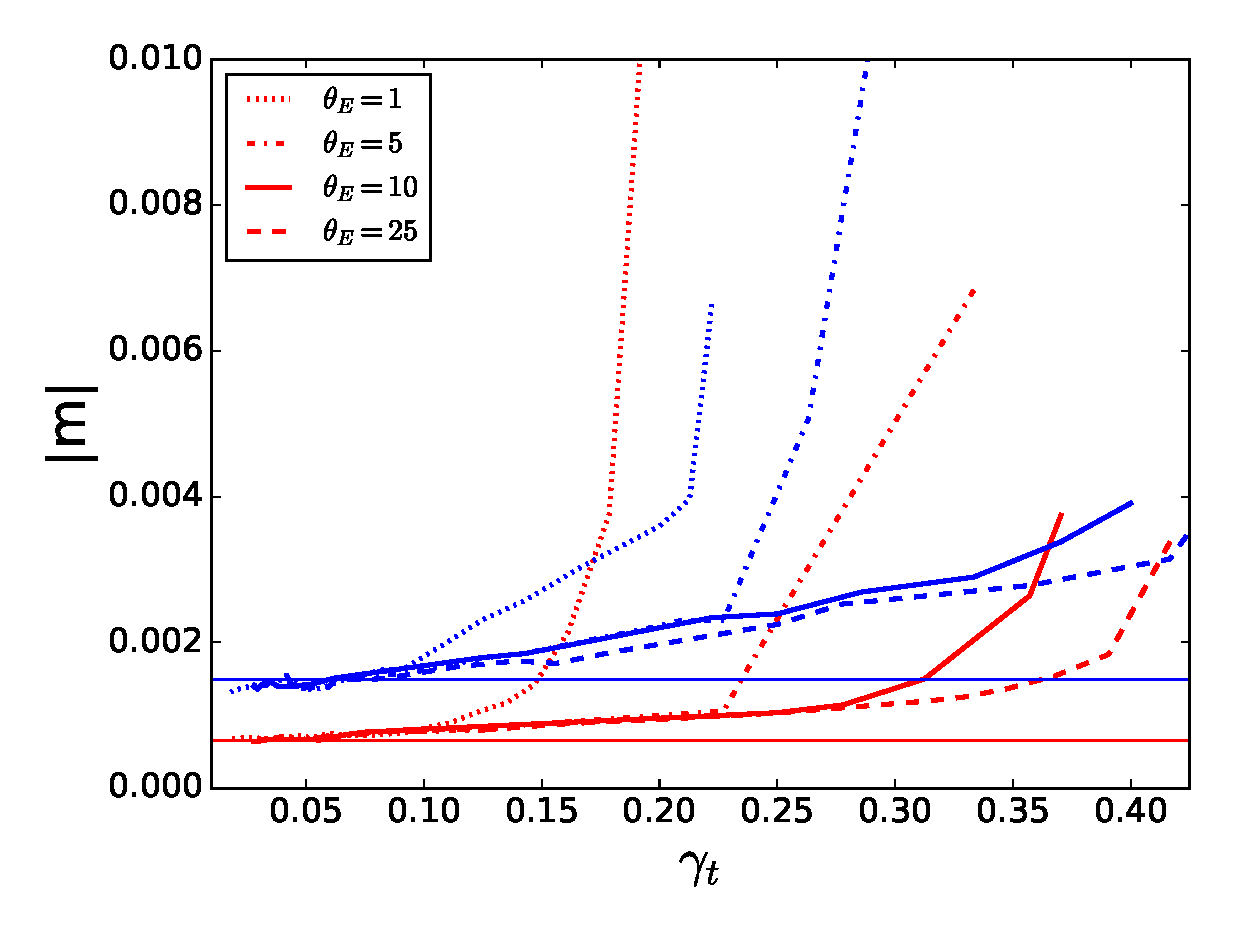
\includegraphics[width=\hsize]{zcg_sis.eps}}
  \caption{The CG bias versus tangential shear in complete lensing
    process (solid lines). The dotted lines correspond to the results
    from only shear process. }
  \label{fig:biasofgamma}
\end{figure}
%

\subsection{Calibration of CG bias using simulated HST images}
\label{sec:noisy}

The {\it Euclid} observations lack high-resolution multi-band images to measure the CG bias directly for each source galaxy. However, the cosmological lensing signal is typically inferred from the ellipticity correlation function, which involves  averaging the shapes of large ensembles of galaxies. Provided the average bias that is caused by colour gradients is known for a selection of sources, it is possible in principle to obtain unbiased estimates of the ellipticity correlation function. Here it is particularly important that the correction for the average CG bias accounts for the variation in redshift
and colour. The former is relevant for tomographic cosmic shear studies, whereas the latter avoids
significant spatial variation in the bias because of the correlation between galaxy colour, or morphology, and density.

\citetalias{Semboloni13} showed that HST observations  in both the F606W and F814W filters can be used to determine the CG bias to meet {\it Euclid} requirements. However, \citetalias{Semboloni13} did not consider the complicating factor that the HST images themselves are noisy. Although the HST data are typically deeper than the nominal {\it Euclid} data, and the HST PSF is considerably smaller, it is nonetheless necessary to investigate the impact of noise in more detail. We address this particular question here, before we determine the CG bias from actual HST data in Sect.~\ref{sec:candels}.

The method to calibrate the CG bias using observations in two bands is described in detail
in \citetalias{Semboloni13}, but here we outline the main steps for completeness. To model the
wavelength dependence of the image we use two narrow-band\footnote{To distinguish these filters from the broad VIS pass-band we refer to the F606W and F814W as narrow bands, but acknowledge that these are commonly referred to broad-band filters and that genuine narrow-band filters are significantly narrower.} images, each of which is given by:
%
\be
I_i({\bm\theta}) = \int_{\Delta \lambda_i} T_i(\lambda)\, I({\bm \theta},\lambda) \;\d \lambda,
\elabel{linearitp}
\ee
%
where $T_i(\lambda)$ is the transmission of the $i$th narrow filter. We assume that for each pixel the wavelength dependence of the image can be interpolated linearly:
%
\be
I({\bm \theta},\lambda) \approx a({\bm \theta})\lambda + b({\bm \theta}).
\elabel{interpolate}
\ee
%
Eqs.\ref{eq:linearitp} and \ref{eq:interpolate} yield a linear set of
equations on each pixel, which can be used to solved for the
coefficients $(a,b)$:
%
\be
T_{ai} \lambda a(\theta) \,+\,T_{bi} b(\theta) = I_i(\theta), \quad\; i=1,2,
\elabel{lineareq}
\ee
%
where $T_{ai,\,bi}$ is the integrated transmission function at two
filters. With $(a,b)$ and Eq.\ref{eq:interpolate}, one can obtain
approximated galaxy images of each wavelength
$I(\theta,\lambda)$. Then we will follow the same procedure as in
previous section to estimate the CG bias. {\bf need to rephrase and 
think about the notation.}

We first consider the recovery of the CG bias for noiseless observations
of the two reference galaxies. We simulate the images in the F606W and
F814W filters at different redshifts, ignoring evolution in the SEDs. We
adopt the native sampling of the Advanced Camera for Surveys (ACS)
on HST of  $0.05$ arcsec/pixel. As shown in \citetalias{Semboloni13},
we cannot ignore the blurring of the observed images by the HST PSF,
and to mimic this we assume an obscured Airy function for a mirror 
with diameter $D=2.5$ and obscuration  $0.33$ as a proxy for the HST PSF.
We deconvolve our synthetic HST images and create the images at different
wavelengths as the starting point for the flow presented in Fig.~\ref{fig:flowchart}.

Following \citetalias{Semboloni13}, we show the CG bias as a function of redshift
for galaxy `B' (left panels) and `S' (right panels) in Fig.~\ref{fig:biasofz50} . The results for the actual
CG bias are indicated by the solid black lines, whereas the dashed black
lines indicate the recovered values from the noiseless synthetic HST observations
in the F606W and F814W filters. These results show that the CG bias varies
significantly with redshift. The bottom panels show the residuals between the
recovered and the true bias. The residual bias is within the target tolerance for {\it Euclid}, 
indicated by the grey band, for all redshifts.

\begin{figure*}
  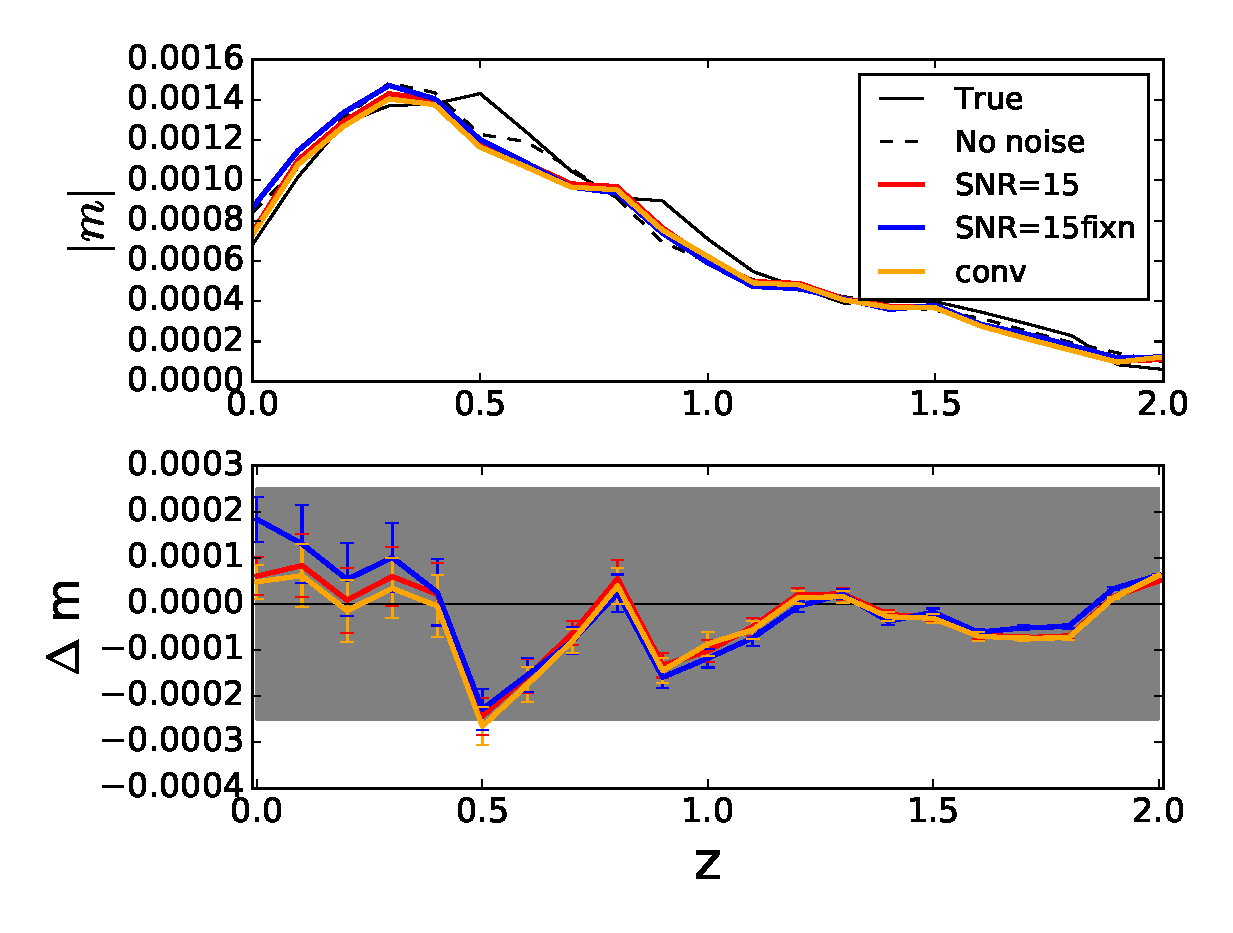
\includegraphics[width=8.0cm]{zs2n_b_snrtt50.eps}
  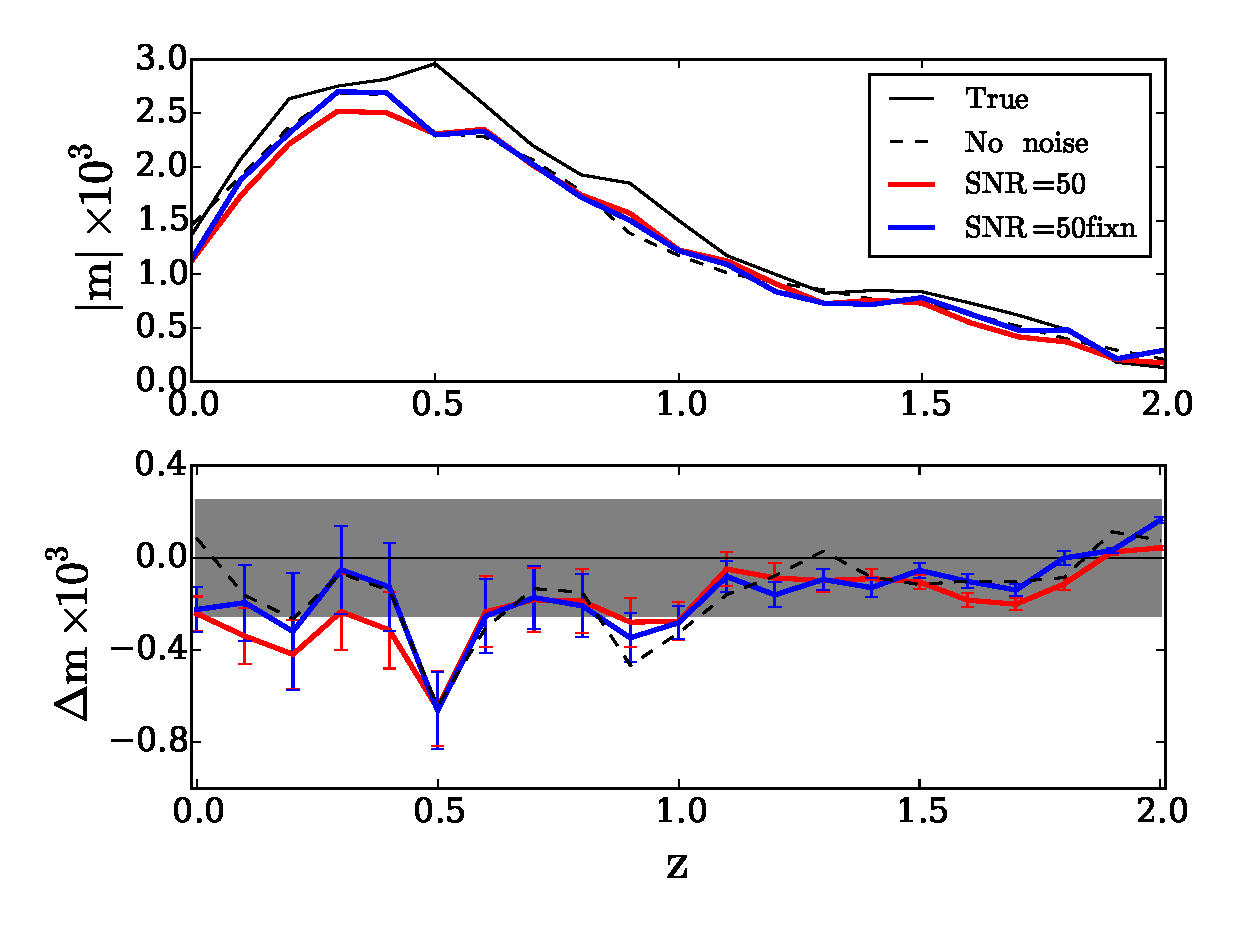
\includegraphics[width=8.0cm]{zs2n_s_snrtt50.eps}
\caption{The multiplicative CG bias as a function of redshift
  for the reference galaxies, with the results for galaxy `B' shown
  in the left panel and those for galaxy `S' in the right panel.
  The dashed black line is the recovered bias when we mimic 
  noiseless HST observations in two filters. The solid red line
  indicates the results when we use the best fit {\sc Galfit} model
  in both filters to estimate the CG bias when the simulated HST images have
  an input SNR$=50$ (averaged over 40 noise realisations at each
  redshift). The blue line shows the results when we fix the Sersic index
  in the fit. The bottom panels show the residuals $\Delta m$ with respect
  to the true CG bias. The grey band indicates the 
  nominal {\it Euclid} requirement.}
\label{fig:biasofz50}
\end{figure*}

This comparison, however, does not account for the fact that the HST images
will contain noise. Although the {\it Eucid} data are shallower, it is important to
quantify the impact of noise on our ability to recover the CG bias using archival
HST data. To do so, we add Gaussian noise to the simulated HST images, where
the r.m.s. noise level $\sigma$ is determined by the signal-to-noise ratio of the galaxy,
SNR, the total flux within an aperture of radius $1.5\,r_{\rm h}$, $F_{\rm tot}$,
and the number of pixels within this aperture, $N_{\rm tot}$, such that
%
\be
\sigma = {F_{tot} \over {\rm SNR} \sqrt{N_{tot}} }.
\ee
%
For reference, we compared the input SNR for the two reference galaxies
to that estimated by {\sc SExtractor} \citep{Bertin96}.
We find good agreement for galaxy `B' for SNR values ranging from 5 to 50
in both HST filters. The agreement is also good for the `S' galaxy, but 
{\textsc SExtractor} returns lower values if the input SNR is larger than 30.
We consider two noise levels: a SNR=50 corresponds roughly to a 
VIS magnitude of $m_{\rm VIS}=23.7$, a bit brighter than the typical
galaxy used in the {\it Euclid} weak lensing analysis; a SNR=15 approximately 
corresponds to $m_{\rm VIS}=25.2$, the faintest galaxies that might be used.

The deconvolution of noisy images is problematic, because the presence of noise
will lead to biased estimates of the underlying galaxy. Instead we regulate the 
problem by assuming that galaxies can be fit by a bulge and disk component,
each described by a Sersic profile. We fit this model, convolved with the PSF, to 
the noisy images in each band and use the best fit model to compute the CG bias. 
To perform the fit, we use {\sc Galfit} \citep{Peng10} with 
the prior constraints on the galaxy parameters (Sersic index, effective radius,
and axis ratio) listed in Table~\ref{fitpar}.
 %
\begin{table}
\begin{center}
\begin{tabular}{ccc|cc}
\hline\hline
parameter &S-606W  & S-814W  & B-606W & B-814W \\ \hline
$n_1$ &0.5-2.5  &0.5-2.5  &0.5-2.5 &0.5-2.5 \\ \
$n_2$ &0.5-2.5  &0.5-2.5  &0.5-2.5 &0.5-2.5 \\ \
$R_{\rm bulge}$ &1-10 &1-10  &3-30  &3-30  \\ 
$R_{\rm disk}$  &5-30 &5-30  &10-60 &10-60 \\ 
$q$      &0.6-1  &0.6-1  &0.6-1 &0.6-1 \\ 
\hline
\end{tabular}
\caption{\label{fitpar} Constraints for the fitting parameters in {\sc Galfit}.
The first two columns are for two images of the S-galaxy, the other two are
the image of B-galaxy.
$n_1$ is the Sersic index for bulge, and $n_2$ is the Sersic index for disk.
The effect radius is given in unit of pixel ($0.05$ arcsec).}
\end{center}
\end{table}

We use combine the images in the two filters and use {\sc SExtractor}
to estimate the center and some initial galaxy parameters that are used
as the starting point by {\sc Galfit}. The resulting best fit images
depend somewhat on these initial values, and thus could affect the 
estimate for the CG bias. This will be more prominent as the SNR of
the images decreases. To explore this we perform the fits using two
sets of initial parameters: in the first we leave all parameters free,
while in the other case we fix the Sersic index to its simulated value,
but leave the other parameters free.


We use the best fit models to compute the CG bias, following the same
algorithm as was used to compute the signal in the noiseless case. 
We show the resulting average inferred CG bias in Fig.~\ref{fig:biasofz50} for SNR=50 as a function
of redshift for the two reference galaxies (`B' in the left panel and `S' in the
right panel). The bottom panels in Fig.~\ref{fig:biasofz50} show the residuals 
$\Delta m$ with respect to the true multiplicative CG bias. To  determine the average
bias we analyse 6 rotations of the galaxy and use the average value as our estimate of 
the galaxy ellipticity \citep{Nakajima07}.  Moreover we create 40 noise realisations for 
each redshift to estimate the statistical uncertainty in our estimate of the multiplicative
CG bias, which is given by
%
\be
\sigma_m= |m| \sqrt{\rund{\sigma_{\rm cg} \langle e_{\rm cg} \rangle \over \langle e_{\rm ncg}\rangle^2 }^2
  + \rund{\sigma_{\rm ncg} \over \langle e_{\rm ncg} \rangle}^2 },
\elabel{sigmam}
\ee
%
where $\sigma_{\rm ncg}$ and $\sigma_{\rm cg}$ are the uncertainties in the average
ellipticities for the images without and with a colour gradient, respectively.

\begin{figure}
  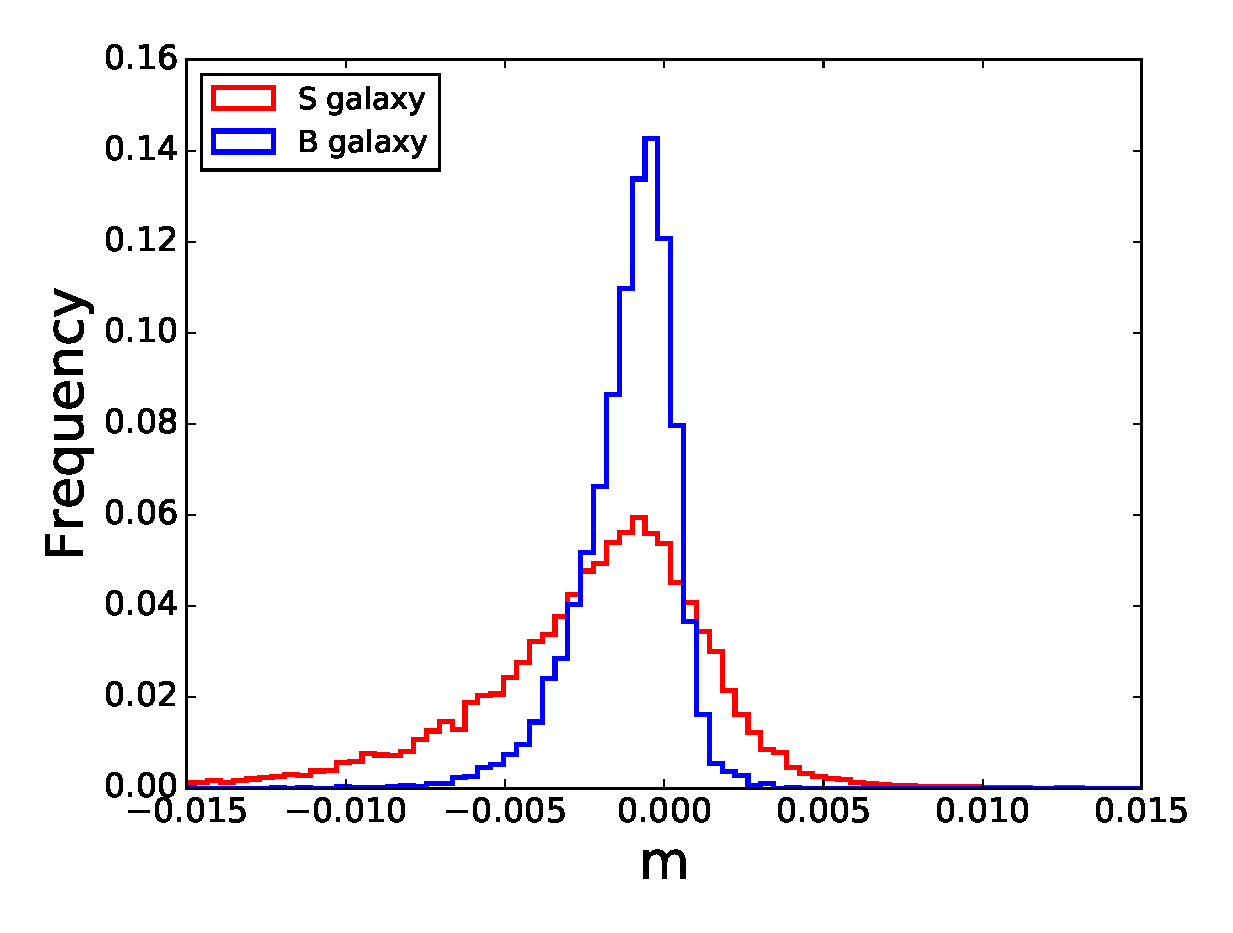
\includegraphics[width=8.0cm]{zs2n15his.eps}
  \caption{Histogram of the inferred CG bias for the `B' (blue) and
  `S' (red) galaxy when narrow band observations with SNR=15
  are used. The histogram combines the results for the different
  redshifts.}
  \label{fig:histogrambias}
\end{figure}
We find that fixing the Sersic index (blue line) or leaving all parameters free (red line)
results in a similar CG bias as a function of redshift. Moreover, the results
closely resemble the noiseless case (dashed lines).  The residuals
presented in the bottom panel of Fig.~\ref{fig:biasofz50} show that 
for the SNR=50 case, we expect that the average CG bias can be determined with an
overall accuracy that meets the adopted {\it Euclid} tolerance, indicated by the grey band.



\begin{figure*}
  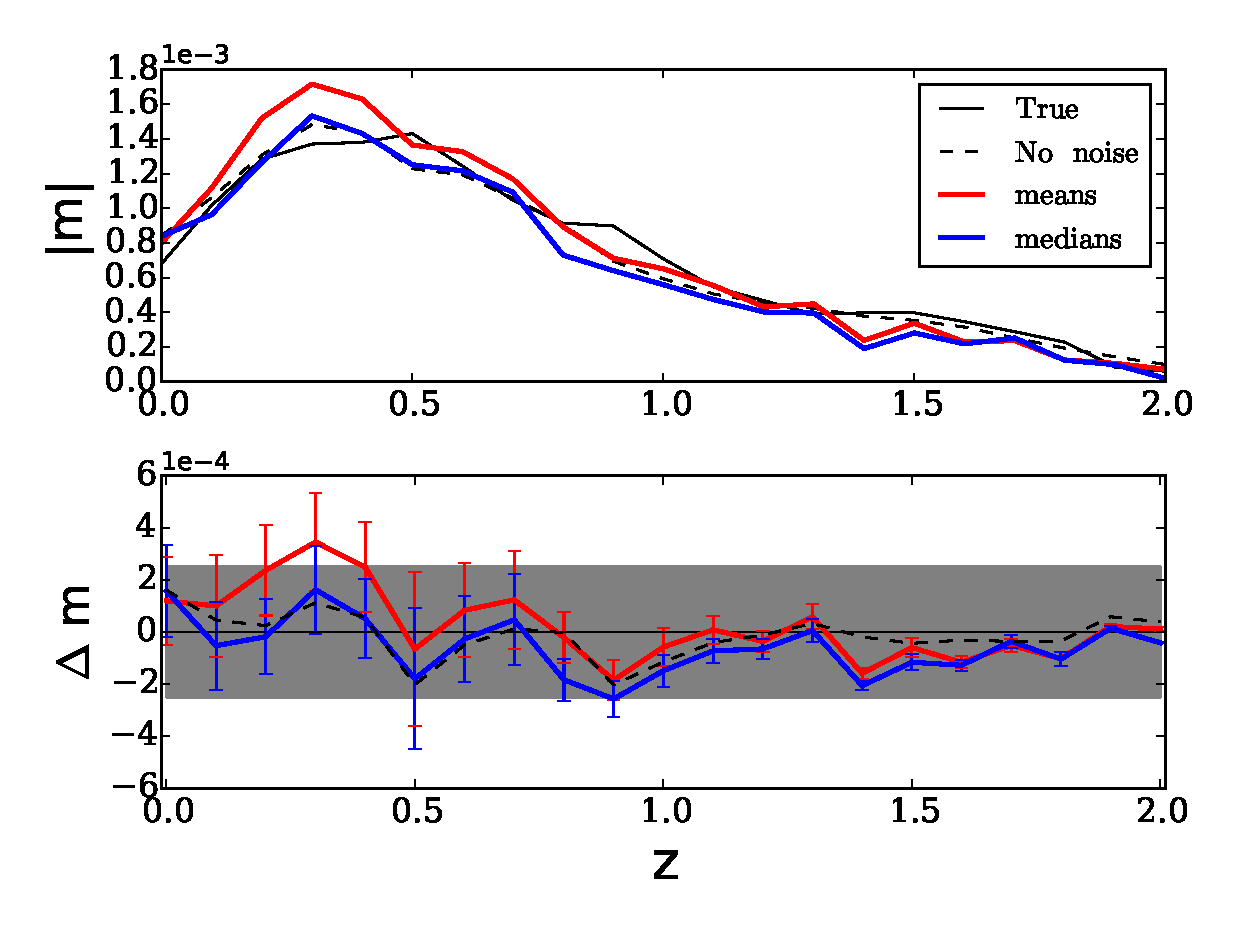
\includegraphics[width=8.0cm]{zs2n_b_snrtt15_medians.eps}
  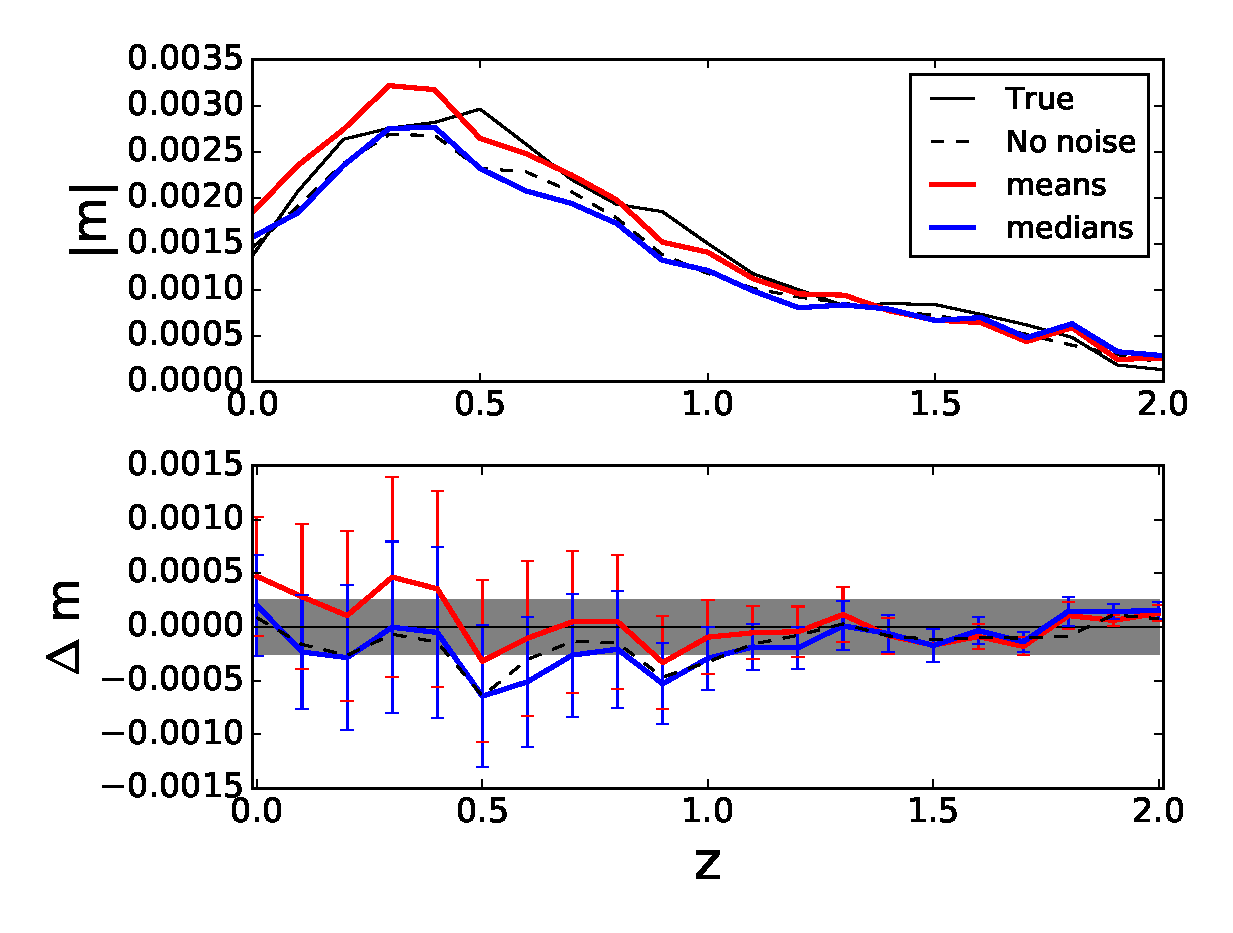
\includegraphics[width=8.0cm]{zs2n_s_snrtt15_medians.eps}
\caption{Same as Fig.\ref{fig:biasofz50} but for images of SNR=15.
  $1000$ realizations are used at each redshift bin for both B- and
  S-galaxy.}
\label{fig:biasofz15}
\end{figure*}
%

Significant deviations occur  at $z=0.5$ and $0.9$, and these can be understood
because the adopted SED of the disk (Irr) contains strong emission lines 
\citepalias[see Fig.~1 in][]{Semboloni13}. These lines enter and exit the F606W filter
at these redshifts, respectively, and the linear approximation for the wavelength
dependence fails. In these, albeit extreme cases, two-band imaging may not
be sufficient. To what extent this will affect the estimate of the CG bias requires
further study.



Figure~\ref{fig:histogrambias} shows the distribution of biases (combining results for the
full redshift range) when the galaxies are detected in the narrow-band images with SNR=15.
The distribution is skewed and especially for the `S' galaxy quite broad. Therefore we 
increased the number of noise realisation to 1000 to ensure robust estimates of the average
CG bias as a function of redshift. The resulting CG bias as a function of redshift are shown
in Fig.~\ref{fig:biasofz15}. We also show the median bias as a function of redshift, which
is slightly different, because the distribution itself is skewed. Nonetheless the bias is
recovered to a level that is acceptable for {\it Euclid}. 




\subsection{PSF variations in calibration data from HST}

So far we implicitly assumed that the simple axisymmetric PSF used to mimic the HST data
is perfectly known. In reality, however, the HST PSF is more complex, and varies spatially
and as a function of time. The small field-of-view of ACS leads to a typically a small number
of stars that can be used to model the PSF.  We therefore examine how well the HST PSF 
properties need to be determined so that they do not affect the CG bias measurement significantly. 

\begin{figure}
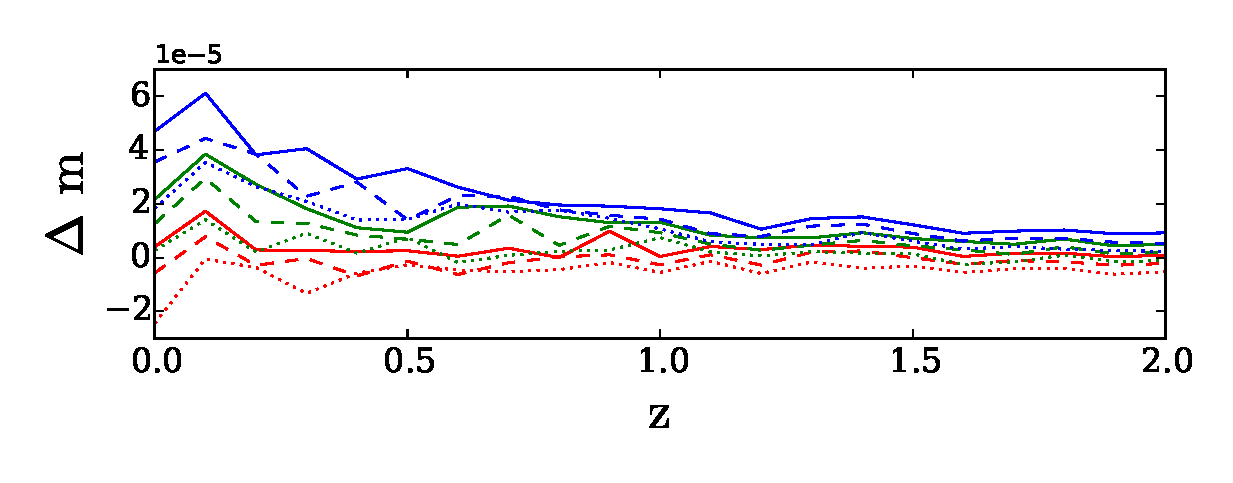
\includegraphics[width=\hsize]{varpsfB.eps}
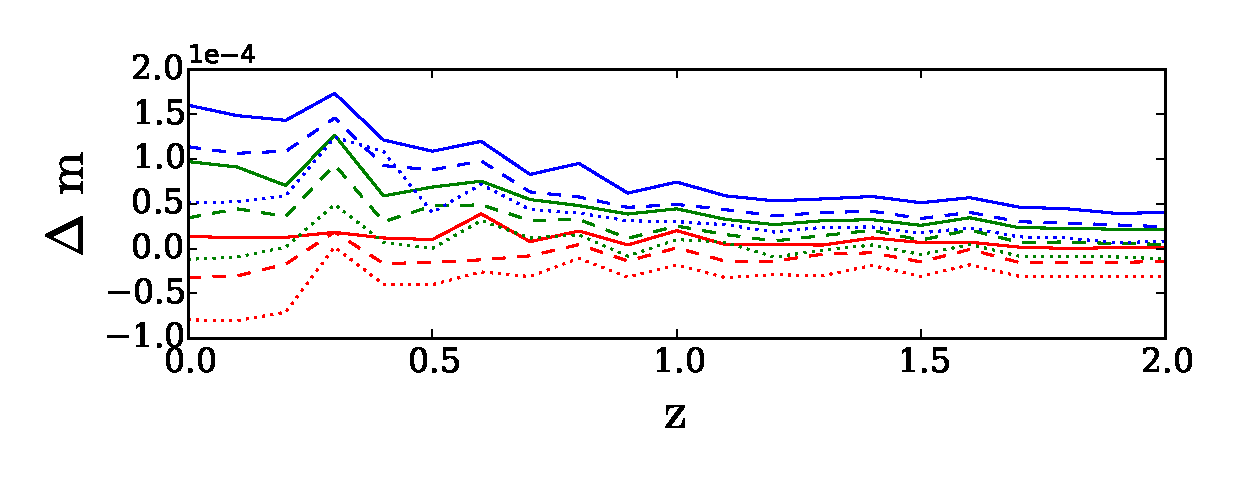
\includegraphics[width=\hsize]{varpsfS.eps}
\caption{Change in multiplicative CG bias when the size of the PSF used in the deconvolution
of the narrow band images is increased (the FWHM differs by 0.9\% between steps). From red, 
green to blue lines, we increase the size of PSF for the F814W filter; from the solid, dashed to dotted 
lines we  increase the size of PSF for the F606W images.}
\label{fig:psfacc1}
\end{figure}

To do so, we generate models where we slightly increase the PSF size in the two bands by computing the 
Airy profile when the wavelength in the calculation is increased by a factor 1.05, 1.10 and 1.15 for the three
cases. This results in increases in the FWHM of 0.9\% between the difference cases.  These models are used 
only in the step where we deconvolve the simulated HST images in the absence
of noise. The change in CG bias, $\Delta m$ as a function of redshift is shown in Fig.~\ref{fig:psfacc1}
for the `B' galaxy (top panel) and `S' galaxy (bottom panel).  The results for an increase in the PSF size in 
the F606W band are indicated by the solid, dashed and dotted lines, respectively; the red, green and blue 
lines indicate the impact of increasing the size of the PSF in the F814W band. The sensitivity to the PSF
errors is typically larger for low redshift galaxies, but the change in CG bias is much smaller than the bias
itself.  As expected, small galaxies are more sensitive to errors in the estimate of the PSF size.


{\bf I do not understand what is done here; why is Tiny Tim used here? I do not understand
why binary stars are introduced. They should not really affect the average PSF model in this
case, but only individual stars. If we want to study this we need realistic distribution, but
the HST stars are faint, and hence distant, and so binary stars are less of an issue anyway.}


To test the impact of imperfect PSF modelling, we make two
comparisons: Comparing a control set of ``actual'' PSFs to a mock set
of stars using these PSFs, including some unresolved binaries; and
comparing the stars in actual images to the best-fit models. In the
former case, we generate mock star fields using PSFs generated with
the TinyTim tool \citep{2011SPIE.8127E..0JK} and allow 30 per cent of
stars to be unresolved binaries, with another star laid on top of them
within a radius of one pixel. In the latter case, we use actual star
fields observed with HST and try two methods of fitting the model to
the stars. In both cases. we perform this for both the F606W and F814W
filters.

The model PSFs are generated using the default parameters for TinyTim
where possible, and the appropriate camera, detector, and filter
passband settings for each image. For the rest of the options, we use:
\begin{itemize}
  \item \textbf{Position on Detector:} Chosen for each star based on its
detected position.
  \item \textbf{Spectrum:} 1; 15 (Use the K7V spectrum, which is chosen
to represent a typical star in the sample. The choice of a fixed
spectrum for stars was found to have a negligible impact on the
models.)
  \item \textbf{PSF Diameter:} 2.0 arcsec
  \item \textbf{Focus-Secondary Mirror Despace:} Fit per image. As HST
    ``breathes'' due to its varying angle relative to the Sun, the
    position of the focus relative to the secondary mirror changes
    over time and cannot be perfectly predicted for any given
    observation. We thus have to fit the best focus position by
    simulating multiple sets of PSFs for each image.
  \item \textbf{Zernike Polynomials:} In the first test, ``focus
    only'', set to default values. In the second test, ``all
    parameters'', these are fit in addition to the focus despace.
  \item \textbf{Subsampling Factor:} $8\times$
\end{itemize}

Stars are selected such that they have a signal-to-noise ratio of at
least $50$, there are no detected objects within $1$ arcsecond ($20$
pixels), and outlier rejection is performed in the fitting procedure.
The stars are normalized and then stacked using inverse-variance
weighting. The corresponding model PSFs are stacked using the same
weights.

%



%
\begin{figure}
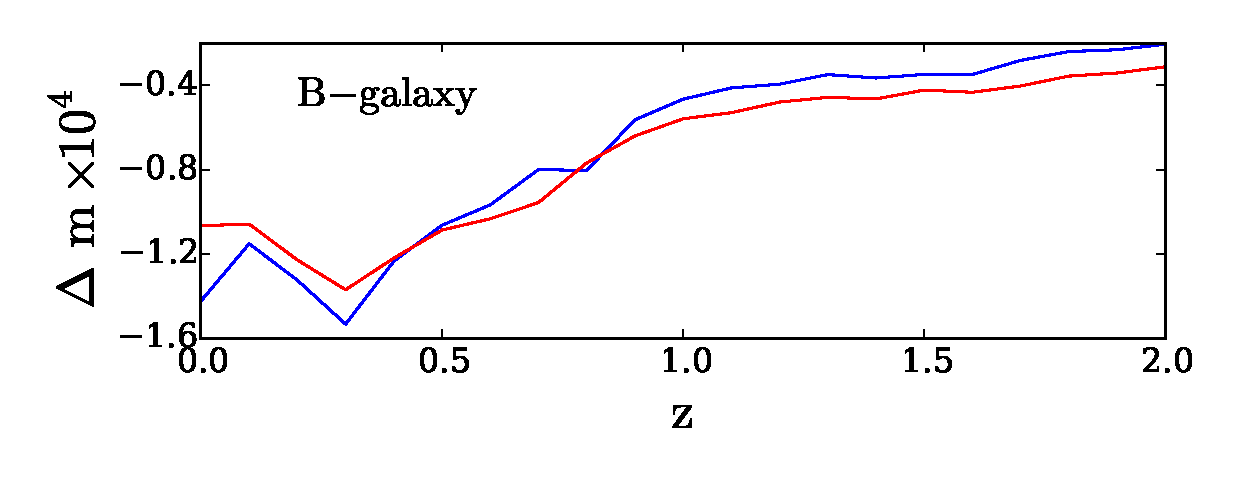
\includegraphics[width=8.0cm]{ztinytim_b.eps}
%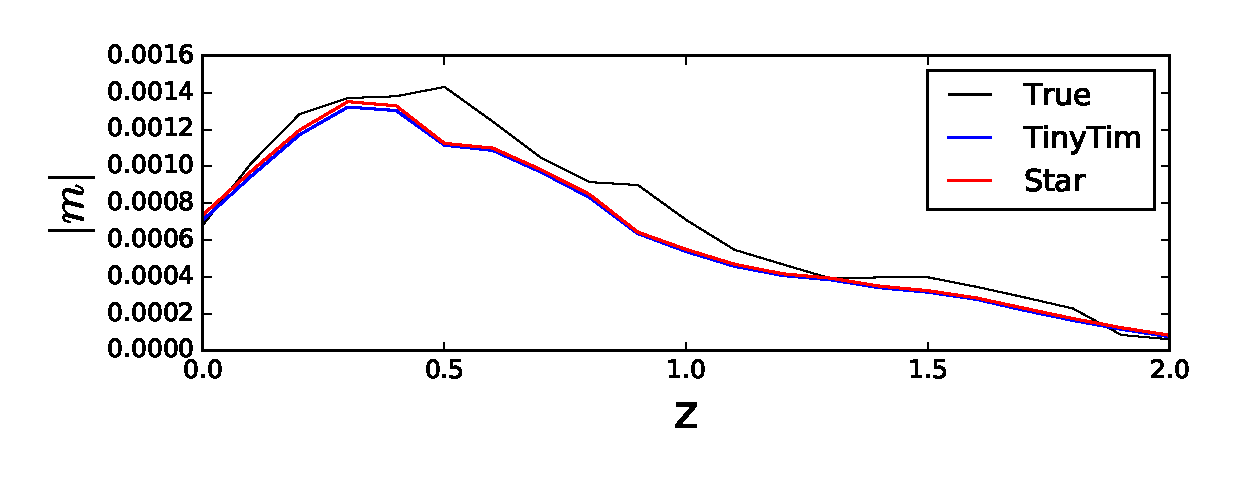
\includegraphics[width=8.0cm]{z_b_bryan2.eps}
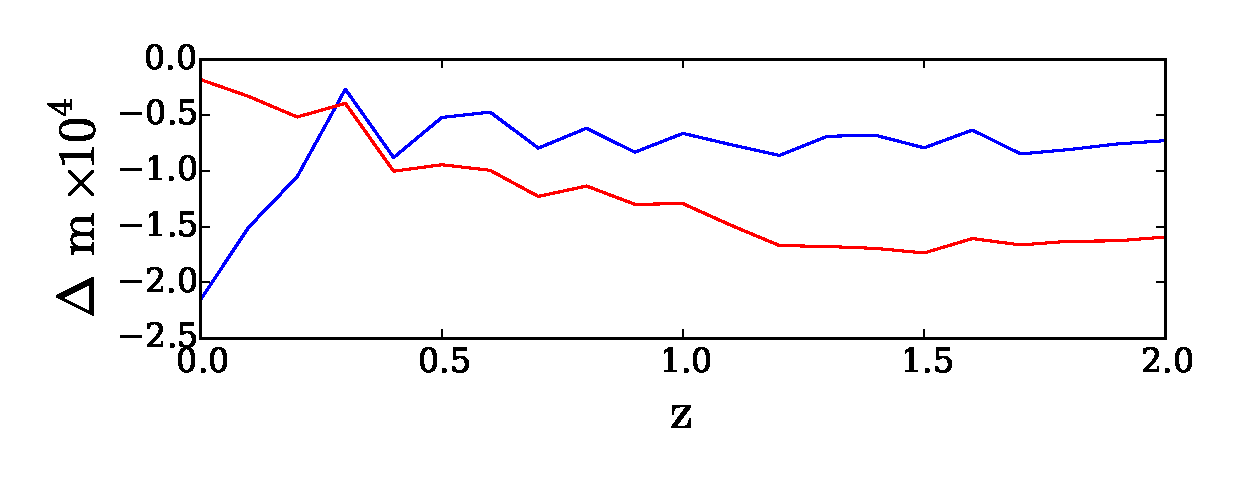
\includegraphics[width=8.0cm]{ztinytim_s.eps}
%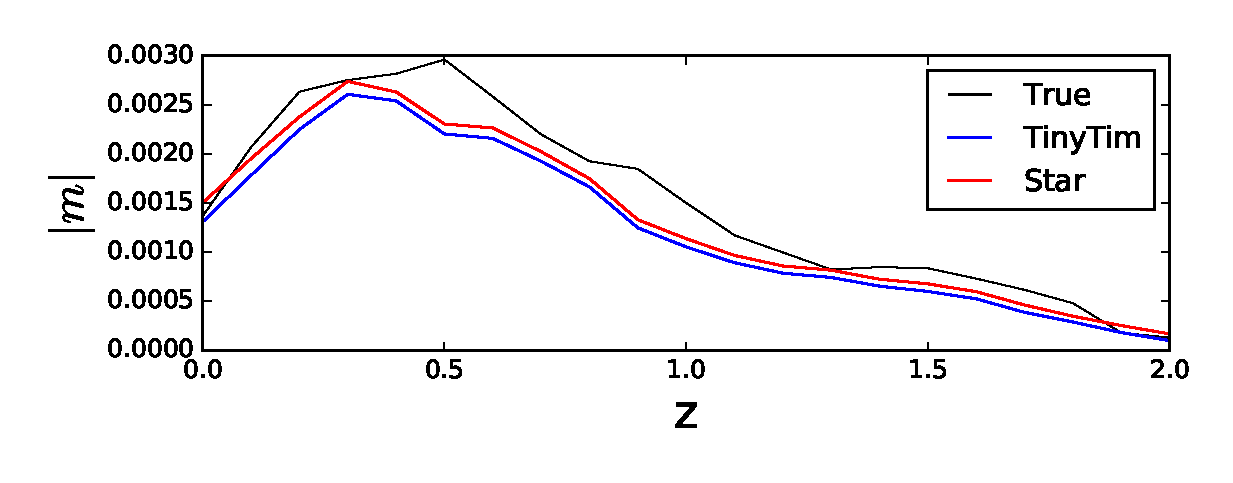
\includegraphics[width=8.0cm]{z_s_bryan2.eps}
\caption{Comparison of PSF between TinyTim model and stars.
  Top (Bottom) is for the B-galaxy (S-galaxy). The solid (dashed) 
  lines are the result using undrizzled (drizzled) PSF. 
  The dotted lines are that if we also include binary PSF effect.}
\label{fig:psfacc2}
\end{figure}
%
In Fig.\ref{fig:psfacc2}, one can see that the inaccuracy of PSF can
cause error on the estimation of CG bias. For the small size galaxy,
the error can reach about $15\%$ for undrizzled PSF, while for the big
galaxy, the error is only a few percent, can be neglect. In the result
using drizzled PSF, the difference becomes smaller. The most
problematic PSF will be those from binary stars. One can see for both
big and small galaxies, we have a significant error.

\section{Measurement from HST observations}
\label{sec:candels}

In the previous section we confirmed the conclusion from \citetalias{Semboloni13} 
that it is be possible to determine the CG bias from HST observations in the F606W 
and F814W filters. Importantly, we demonstrated that the presence of noise in the 
actual data should not bias the results significantly. We therefore proceed now to
determine the expected CG bias in {\it Euclid} shape measurements using
 realistic galaxy populations. To do so, we employ HST/ACS data taken in the F606W and F814W
filters in the three CANDELS fields (AEGIS, COSMOS, and UDS), which have
a roughly homogeneous coverage in both bands \citep[see][]{davis2007,grogin2011,Koekemoer11}.

\subsection{Analysis of CANDELS data}

We base our analysis on a tile-wise reduction of the ACS data, incorporating pointings
that have at least four exposures to facilitate good cosmic ray
removal, yielding combined exposure times of 1.3-2.3ks in F606W and
2.1-3.0ks in F814W.  We employ the updated correction for
charge-transfer inefficiency from \cite{massey2014},
\texttt{MultiDrizzle} \citep{koekemoer2003} for the cosmic ray removal
and stacking, as well as careful shift refinement, optimised
weighting, and masking for stars and image artefacts as detailed in
\cite{schrabback2010}.  Schrabback et al. (in prep.) describe the
generation of weak lensing catalogues for these images.  We base our
analysis on the galaxies passing their source selection and apply
additional magnitude cuts as detailed below. To investigate the
dependence of the colour gradient influence on galaxy colour and
redshift, we match this galaxy catalogue to the photometric redshift
catalogue from \cite{skelton14}.  We list the total non-masked areas
in which these catalogues overlap in Table \ref{table:mag}.

\begin{center}
\begin{table}
  \begin{tabular}{lllll}
    \hline
    Field   &Area (arcmin$^2$) &$N_1$ &$N_2$ &$N_3$\\
    \hline
    AEGIS   &180   &2094  &2112  &3460\\
    COSMOS  &139   &1593  &1656  &2449\\
    UDS     &146   &1455  &1497  &2341\\
    Total   &465   &5142  &5265  &8250\\
    \hline
  \end{tabular}
  \caption{\label{table:mag} Size of the HST CANDELS data sample in F606W
    and F814W bands.  The number of galaxies are shown in three selection
    methods to match the Euclid survey, $N_1$: $m_V<25$ and $m_I<24.5$,
    $N_2$: $m_{VIS}<24.5$, $N_3$: $m_V<25.5$ and $m_I<25$. }
\end{table}
\end{center}
%

We match the galaxy from F606W and F814W bands by selecting that
the difference of galaxy coordinates in two bands is smaller than 1
pixel ($0.05$ arcsec). Moreover, in order to resemble the {\it Euclid} 
wide survey, we apply a selection based on the magnitude of two bands. In the
first selection, the galaxy must be brighter than magnitude $25$ in
the F606W band and $24.5$ in the F814W band. In the second selection (VIS, N2 sample),
we apply the linear interpolation from F606W and F814W band using the
effective wavelength to approximate the Euclid VIS magnitude, and
select the galaxy brighter than $24.5$ in VIS. In the last one (N3
sample), we enlarge the sample by using lower threshold in two bands:
$25.5$ in V and $25.0$ in I band. The number of galaxies is listed in
Table\ref{table:mag}.


{\bf We need to discuss the low number density for the N2 sample; is is low
by a factor 3.}


The galaxy VIS magnitudes will determined by several factors, such as
exposure time and filter transmission, etc. Thus, the actual number of
galaxies can be different from what we have shown in this work. The
approximation that we use rely on the flatness of the source
spectrum. In the VIS sample, the number of galaxies is similar to that in
the first selection in all three fields, which suggest that the
spectra of our galaxies are relatively smooth. In the N3 sample the galaxy
number is much higher.
%
The total galaxy number and number density ($\sim$12/arcmin$^2$) is
lower than that in \citetalias{Semboloni13} for several reasons: we only selected
galaxies for  which the 3D-HST photometric redshift are available, and those
suitable for weak lensing analysis, e.g. the very big or bright
galaxies are not include. Moreover, in \citetalias{Semboloni13} the galaxies are selected
by the magnitude of F814W. However we select galaxies by the estimated
VIS magnitude and well match in F606W and F814W.

There is no significant difference found in the distribution of galaxy
parameters, such as effective radius, axis ratio, photometric redshift
and colour (we use $m_{F606}-m_{F814}$ as colour in this work, and
will write as $m_{V-I}$ later). The SNR of most images in VIS sample
are larger than $15$, thus they will be able to provide relatively
stable estimate for CG bias.
%while the low SNR images may suffer from large uncertainty of bias estimation. Thus we only show the result in the VIS sample.

We also compare the galaxies from 3 catalogues (AEIGS, COSMOS, UDS).  In
the distribution of galaxy parameters (Fig.\ref{fig:datapro1}), we
find no significant difference in half light radius ($r_h$), galaxy
axis ratio or redshift distribution. However, in the colour
distribution, there are more blue galaxies (small $m_{V-I}$) in AEGIS,
which is more significant in N3 sample. We will see later that the
colour of galaxy is also related to the CG bias in shape measurement.
%There is slight difference in the SNR of two filters: the SNR of galaxies in AEGIS are larger than the other two in V-band, while smaller in I-band.
%


\begin{figure*}
  \hbox{
    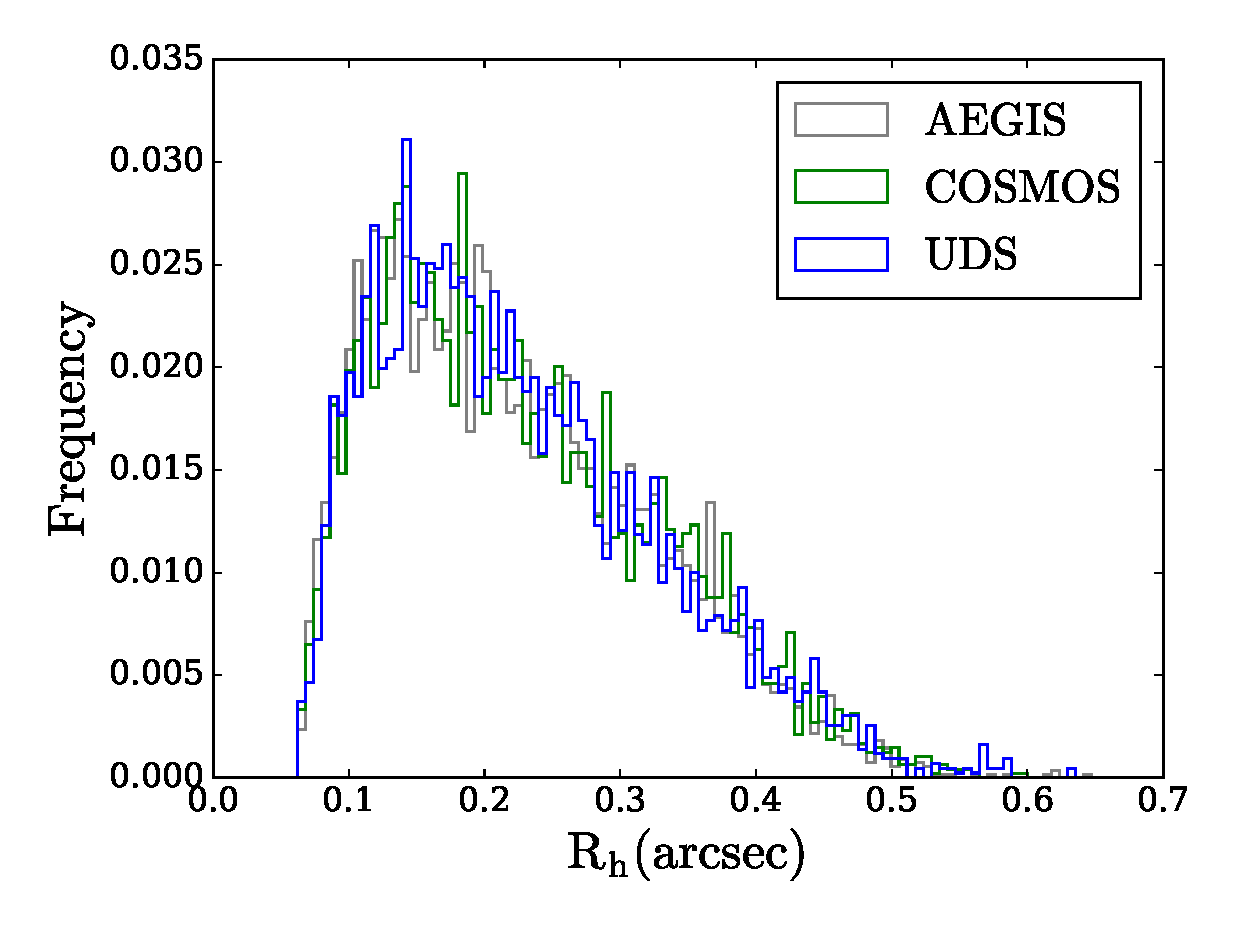
\includegraphics[width=8.0cm]{zhisrh.eps}
    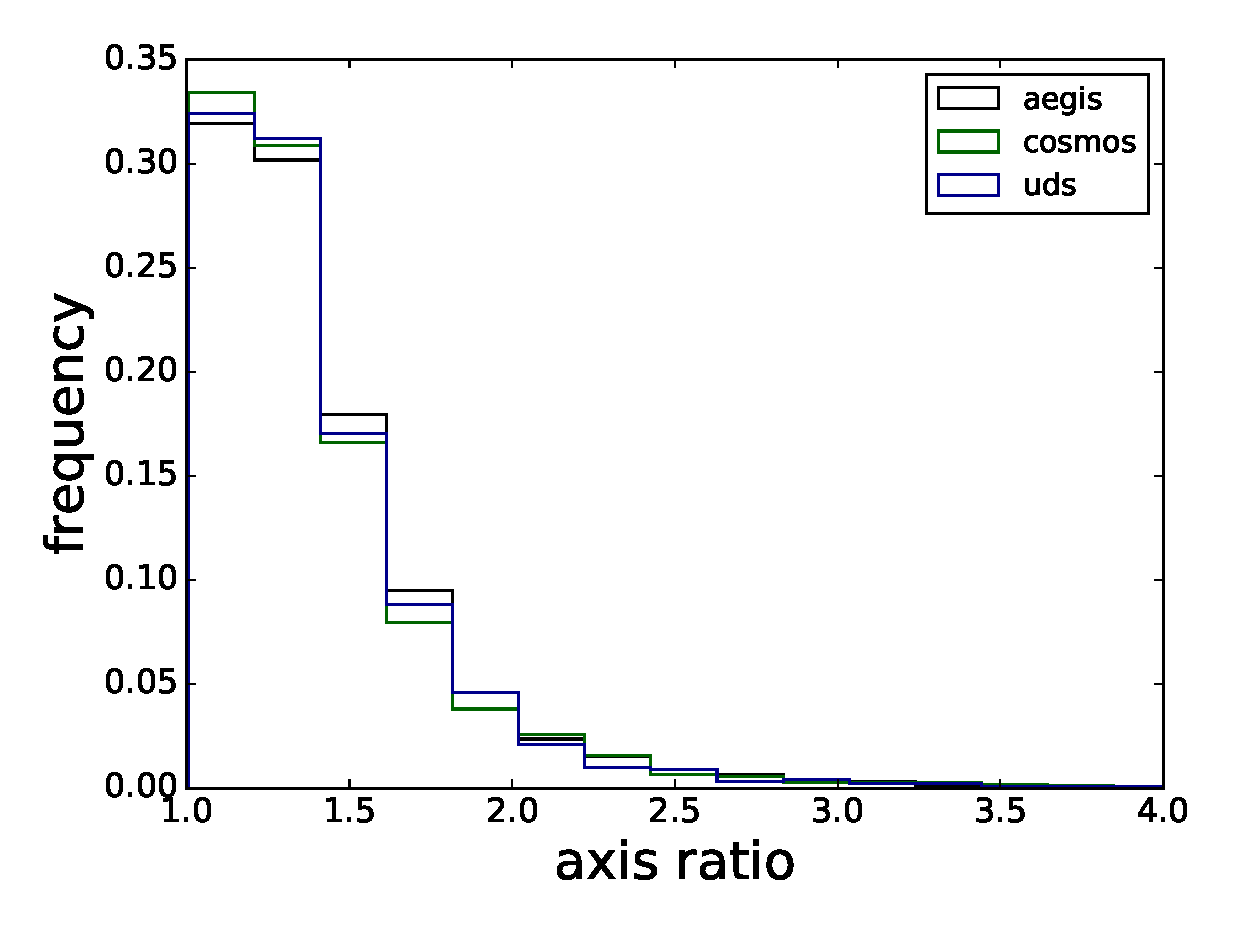
\includegraphics[width=8.0cm]{zhisratio.eps}}
    \hbox{
    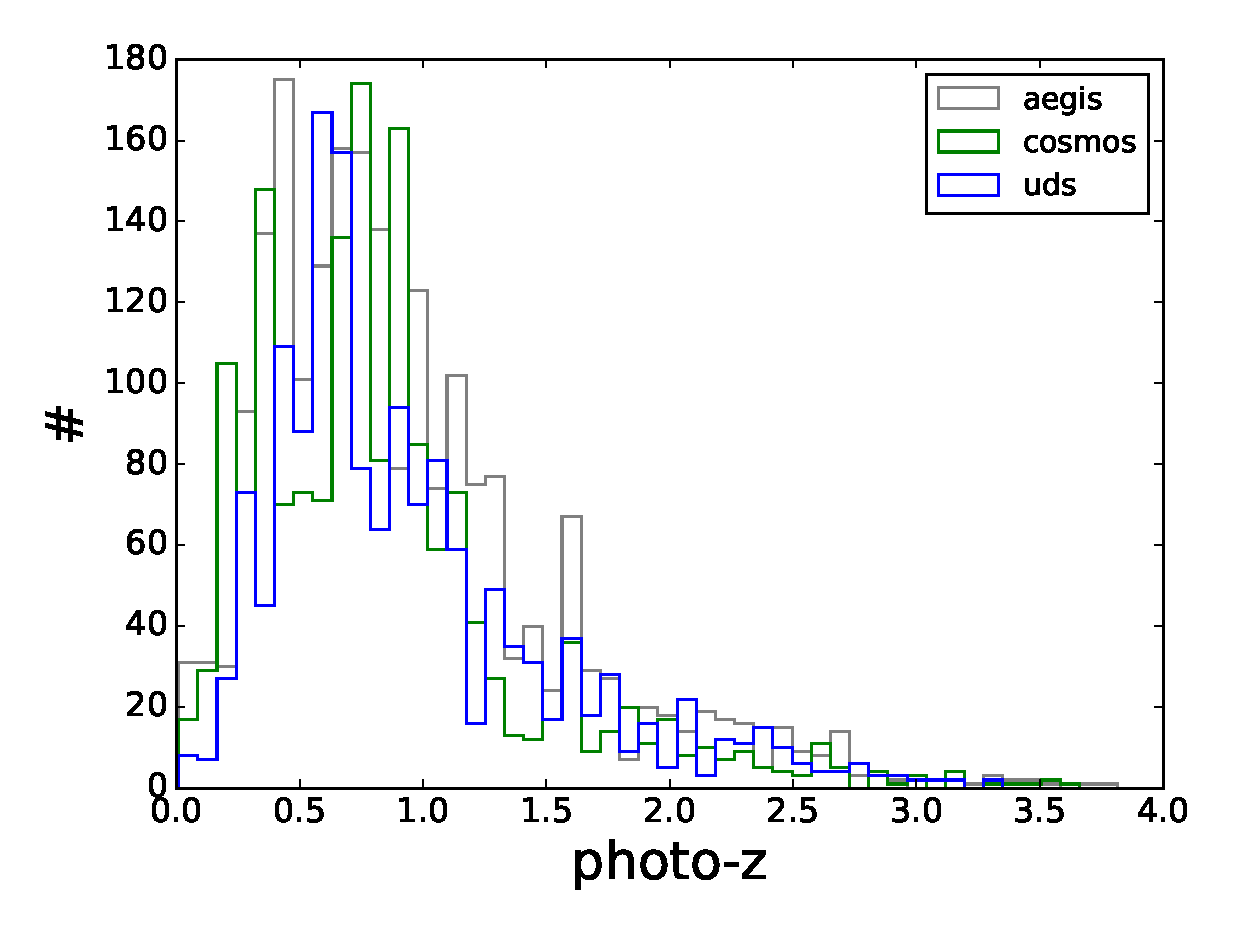
\includegraphics[width=8.0cm]{zhisphotoz.eps}
    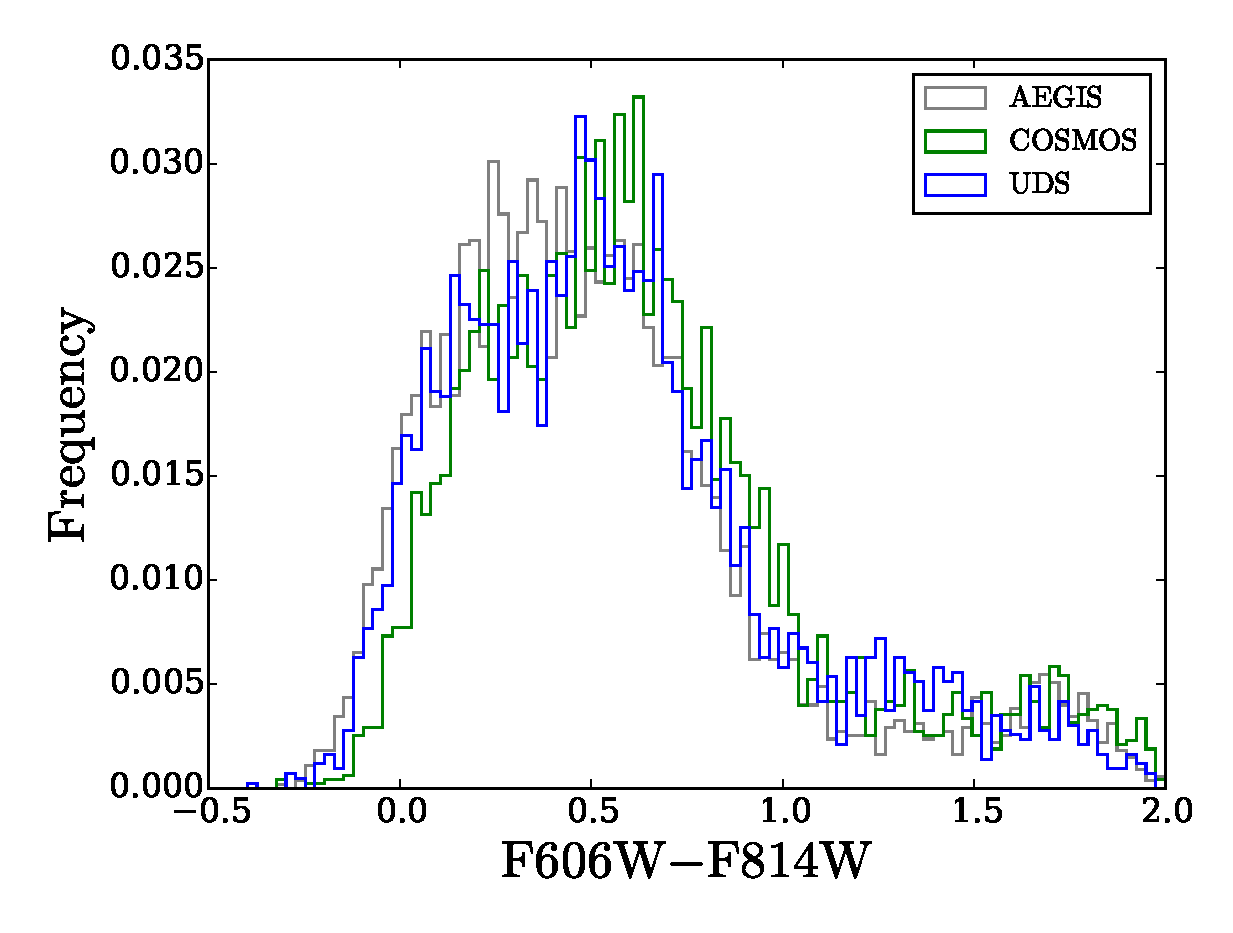
\includegraphics[width=8.0cm]{zhiscolor.eps}}
  \caption{The histogram for basic galaxy properties in our
    sample. The lines with different colours represent galaxies from
    different catalogues (AEGIS, COSMOS, UDS). From left to right: half
    light radius, axis ratio, photometric redshift, and colour
    ($m_{V-I}$).}
  \label{fig:datapro1}
\end{figure*}
%

\subsection{CG bias from CANDELS}

In this section, we use the real galaxy images to estimate the CG bias
which will appear in the Euclid weak lensing survey. For the reference
PSF of Euclid, we use the Airy model (Eq.\,\ref{eq:psfairy}), and we use
the PSF model from TinyTim for the HST data.

We estimate the CG bias following the same procedure for the simulated galaxy:
\begin{itemize}
  \item
    fit the galaxy using one Sersic component for both band
    images. Some constraints such as Sersic index ($0.5<n<5.0$),
    effective radius ($1<r_e<50$ pixel) and axis ratio ($0.6<q<1.0$)
    are adopted in Galfit.
  \item
    interpolate the SED on each pixel of the galaxy image, and
    generate the galaxy at each wavelength (Eq.\ref{eq:linearitp} -
    \ref{eq:lineareq}), and then integrate over the wavelength to
    simulate the CG and NCG galaxy image.
  \item
    measure the shape of two images and calculate the bias $m$. We
    also apply $6$ different orientation of the images in order
    to reduce the intrinsic shape noise.
\end{itemize}
%
In Fig.\ref{fig:cgbhis}, we show the histogram of the CG bias. The CG
bias in most of the galaxies is smaller than $0.01$ ($94\%$). We did
not perform averaging as we did for the simulated noisy images, which
can further reduce the scatter of the bias. Thus the actual bias,
especially the scatter in the sample, is smaller. In the bottom
panel, we estimate the CG bias using a larger weight function
($2r_h$). As one expected, the bias decreases by about one order of
magnitude.

%
%The red line show the CG bias if we perform lensing instead of shearing
%the images. We can see that the bias becomes larger, and the effect is
%stronger than the PSF variations. However, it is highly possible that we
%overestimate the flexion and the effect due to that, since we did not
%consider the real lens property. In the rest, we only show the result using
%shearing.

%
\begin{figure}
  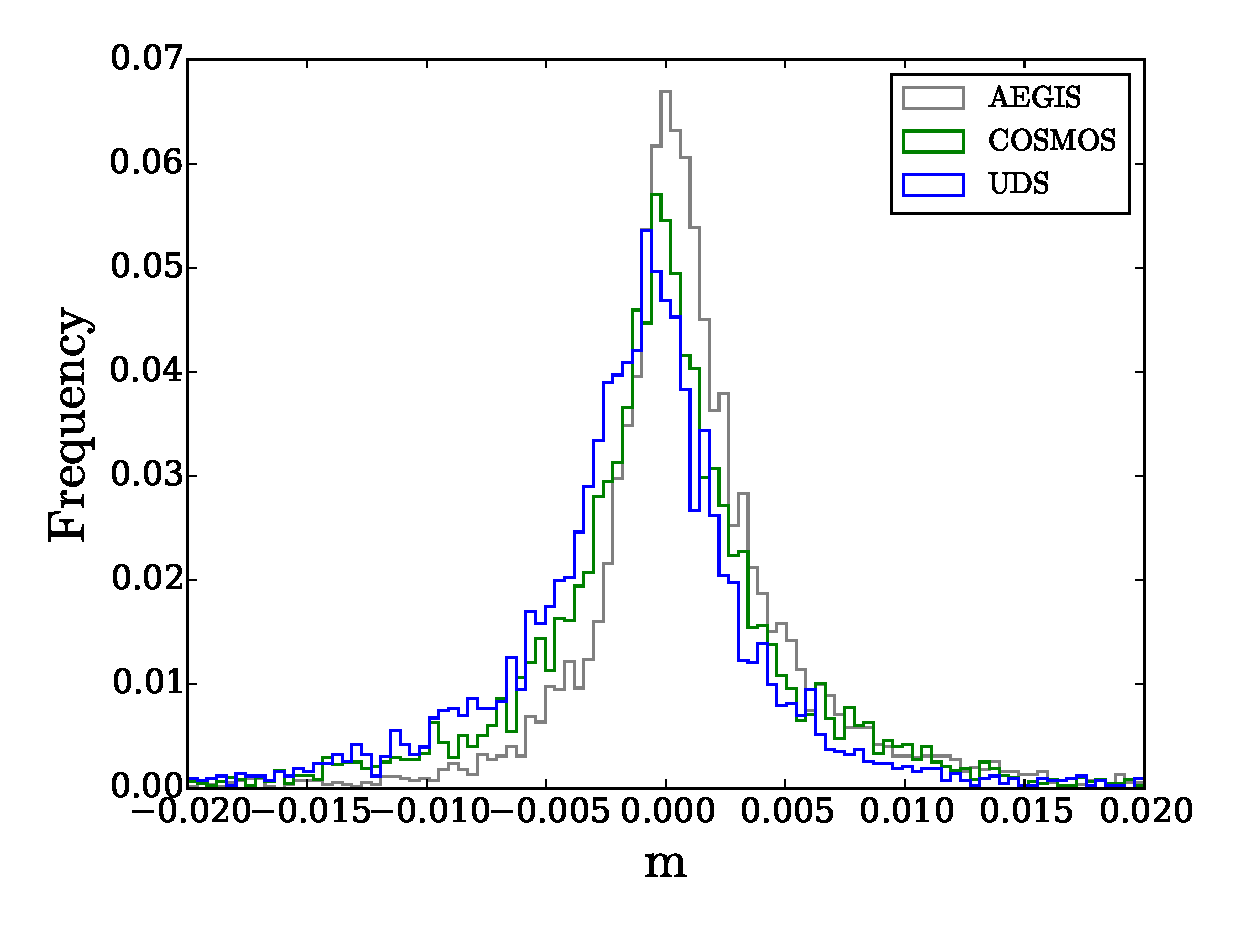
\includegraphics[width=7.0cm]{zhiscgb.eps}
  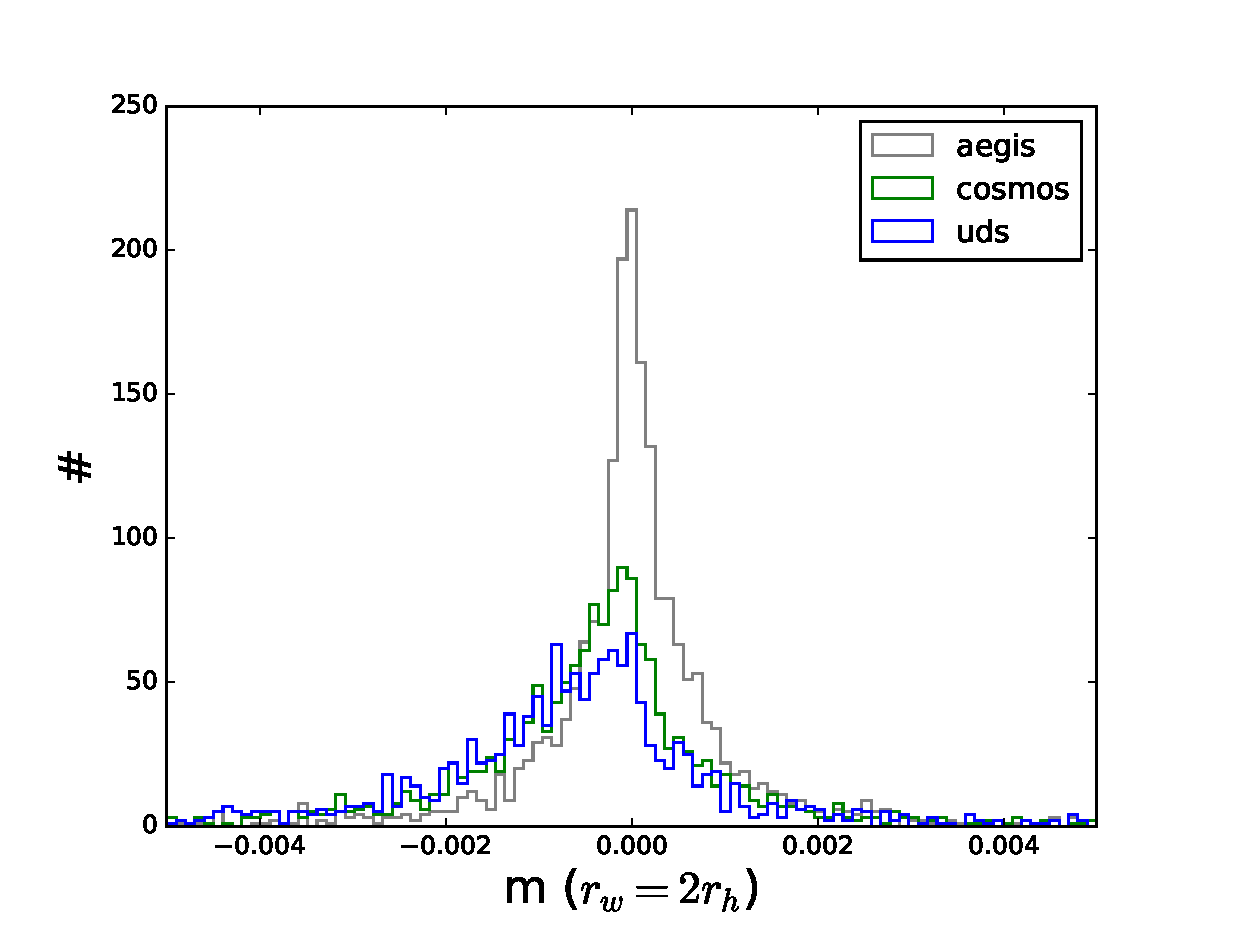
\includegraphics[width=7.0cm]{zhiscgbno.eps}
\caption{CG bias histogram from CANDELS: different colours show the
  result from three catalogues. In the bottom panel we show the CG
  bias using different weight function ($r_w = 2r_h$).  }
\label{fig:cgbhis}
\end{figure}
%
%\begin{figure}
%  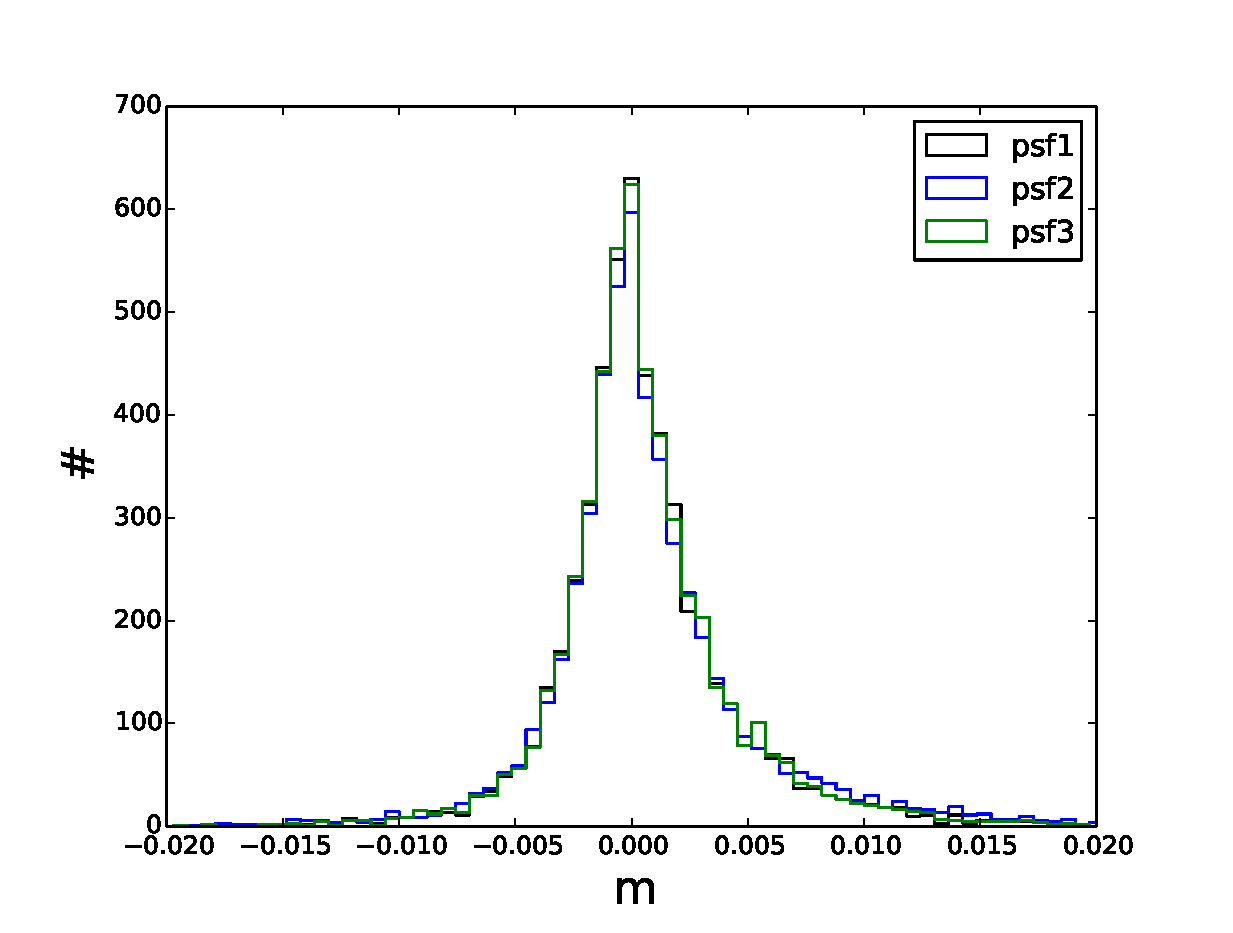
\includegraphics[width=7.0cm]{zcgbhis_psf.eps}
%  \caption{CG bias histogram of CANDELS using three different PSF
%    models from TinyTim.}
%  \label{fig:candelspsf}
%\end{figure}
%
\begin{figure}
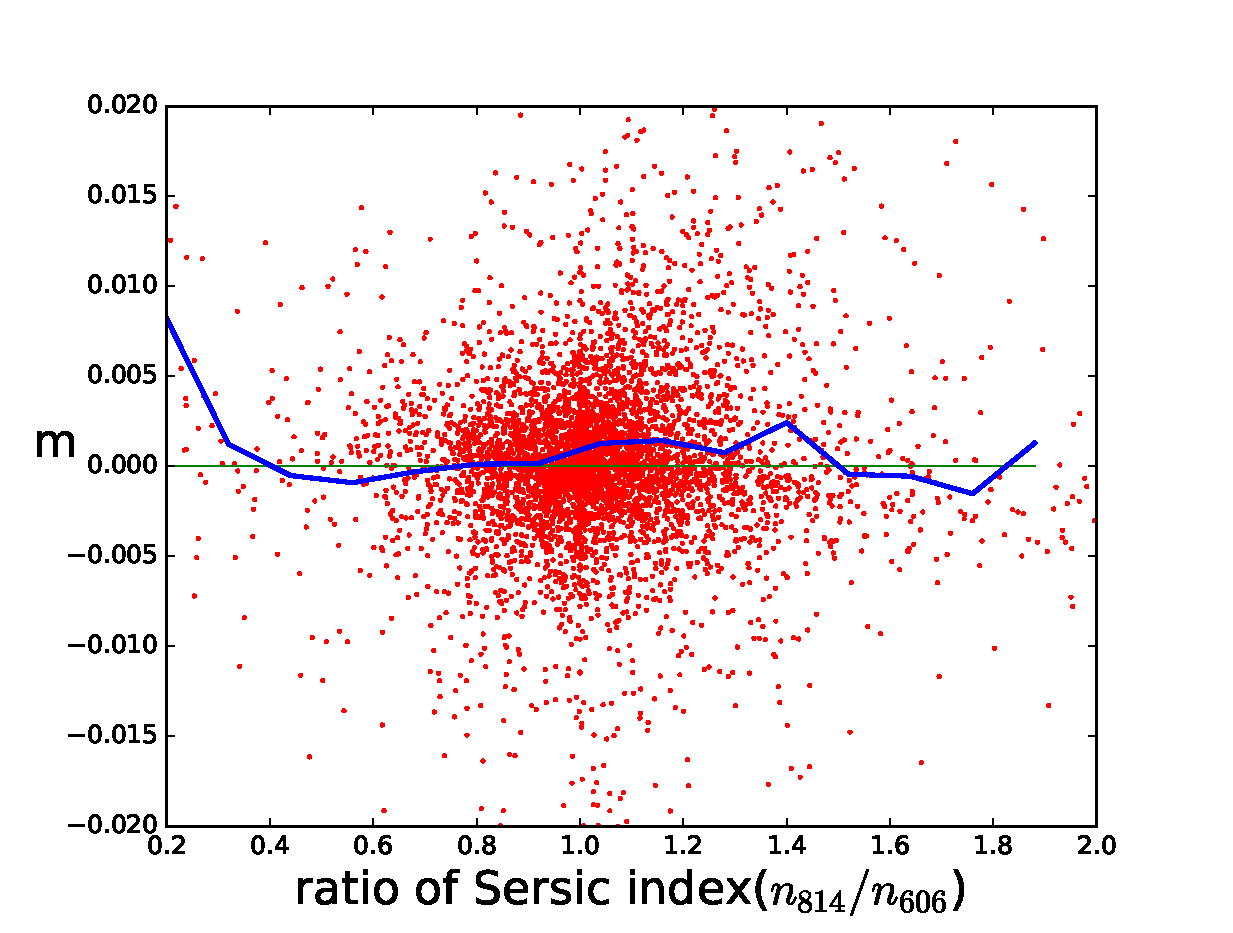
\includegraphics[width=7.0cm]{zcgb-ne17.eps}
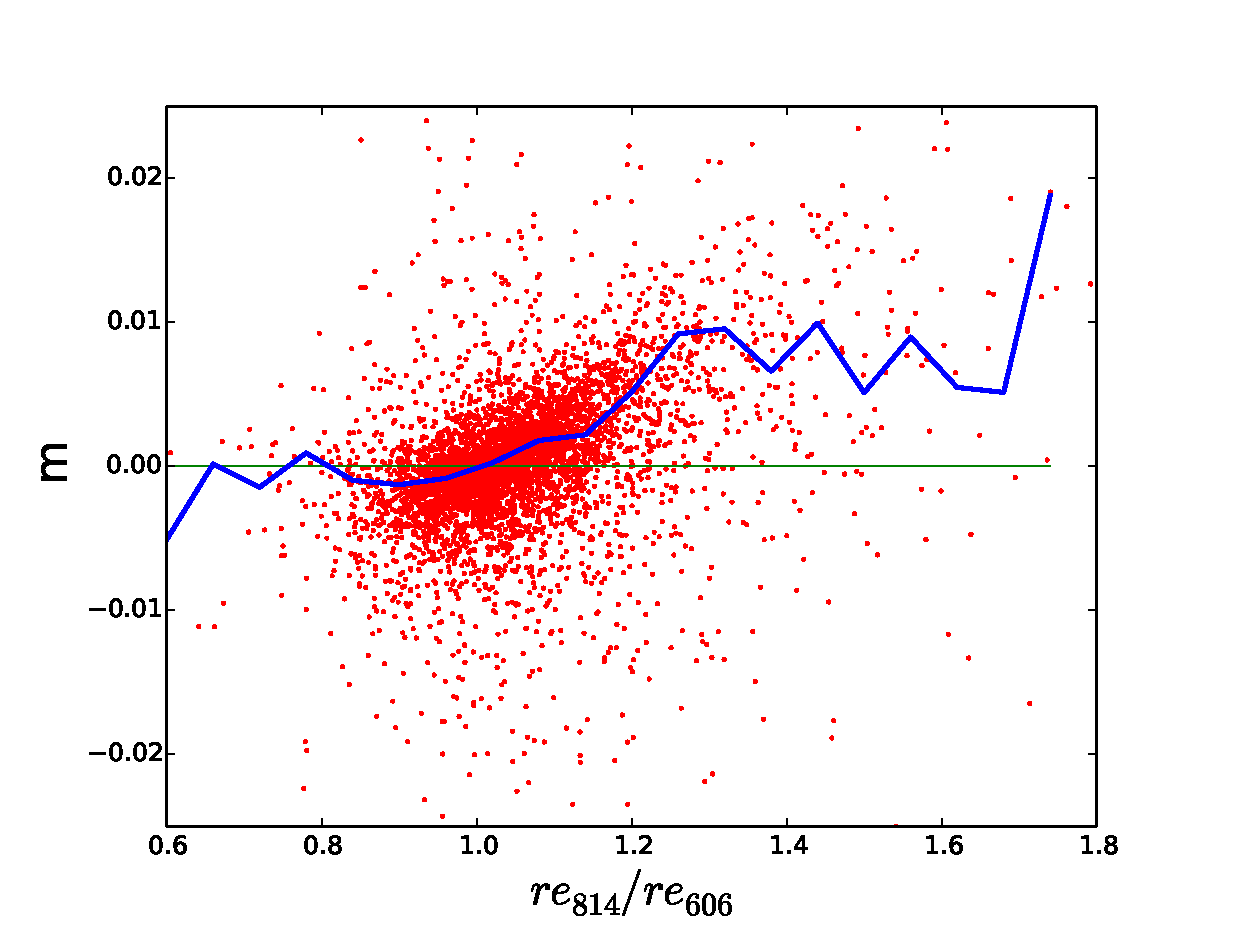
\includegraphics[width=7.0cm]{zcgb-re17.eps}
\caption{CG bias as a function of galaxy properties: ratio of Sersic
  index between two band (top) and effective radius between two bands
  (bottom). The blue lines are the average CG bias over the parameter
  bins.}
\label{fig:cg2fitpar}
\end{figure}
%
\begin{figure}
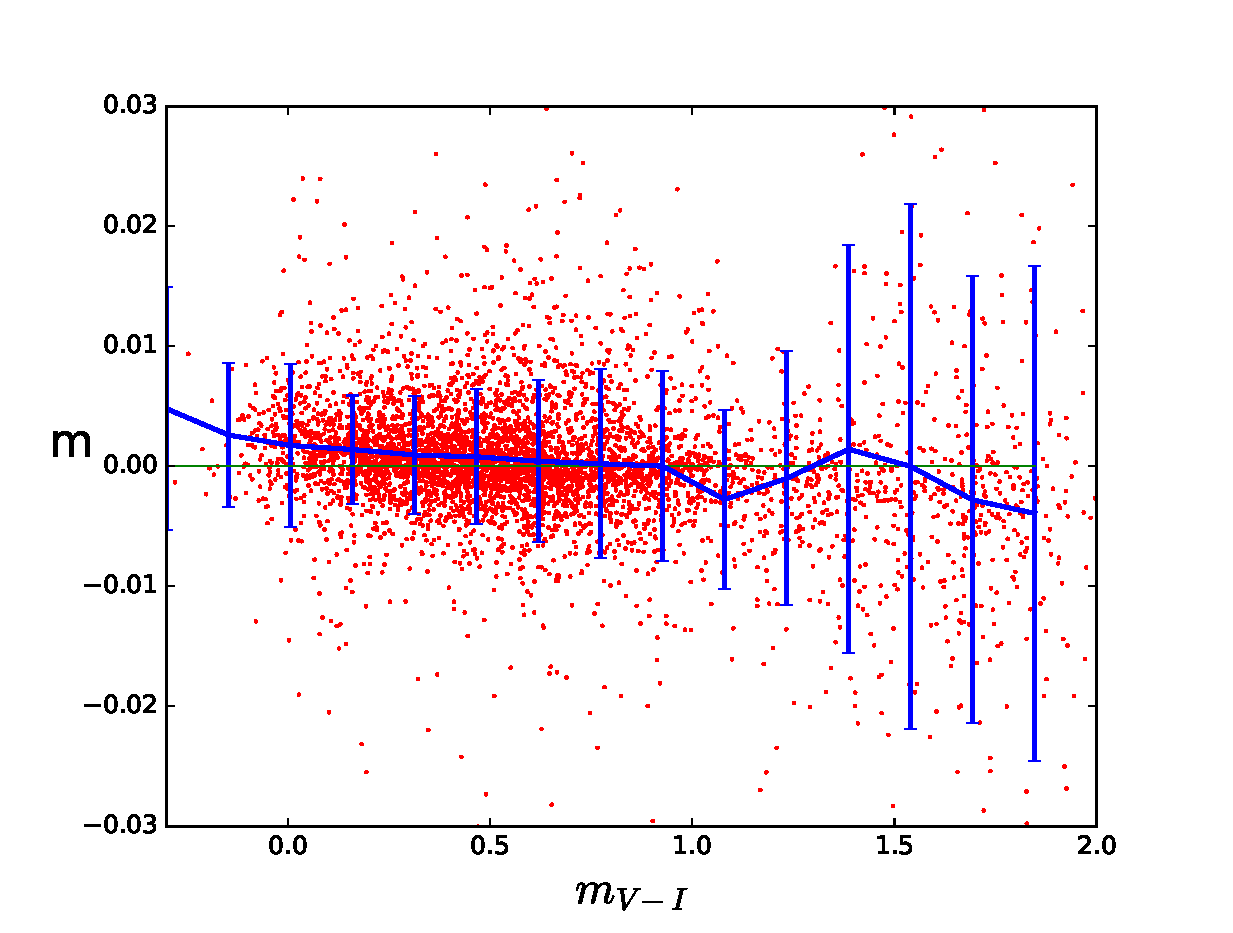
\includegraphics[width=7.0cm]{zcolor17.eps}
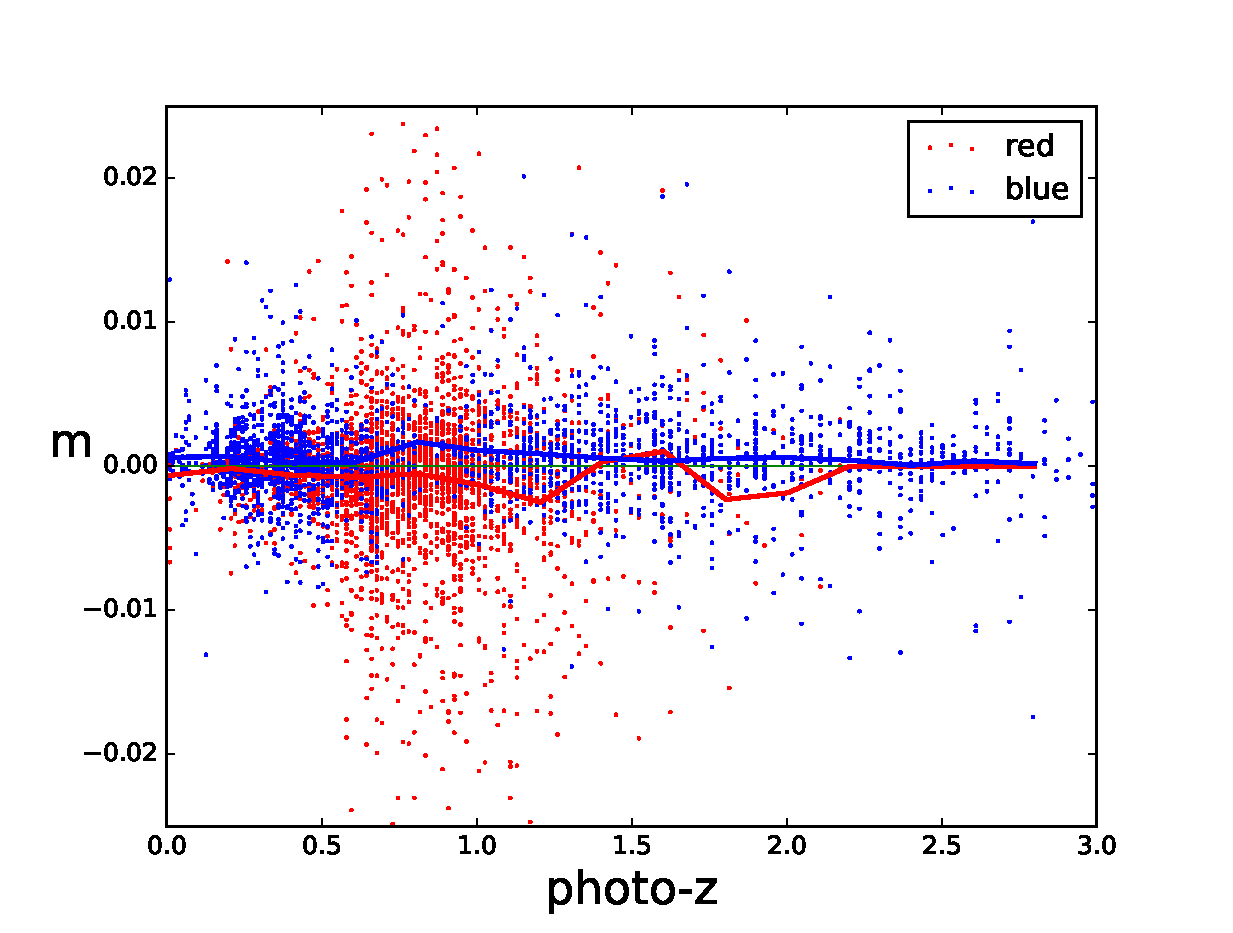
\includegraphics[width=7.0cm]{zphotoz17.eps}
\caption{CG bias as a function of galaxy properties, top: color
  ($m_{V-I}$), bottom: photo-z. In the bottom panel, the red and blue
  points are the bias for red ($m_{V-I}>0.5$) and blue ($m_{V-I}<0.5$)
  galaxies respectively. The lines are the average CG bias in the
  redshift bins.}
\label{fig:cg2color}
\end{figure}
%
\begin{figure}
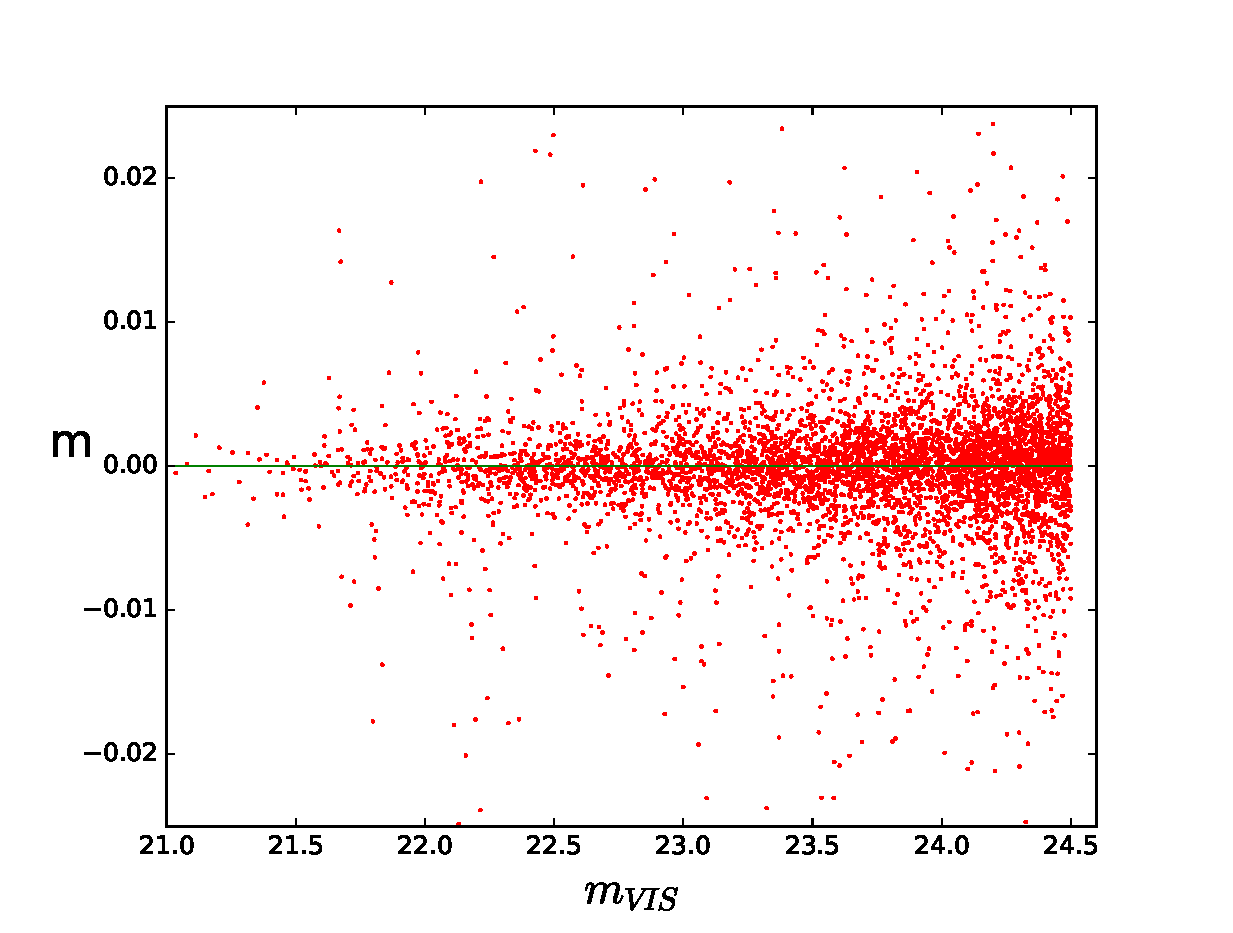
\includegraphics[width=7.0cm]{zcgb-magt17.eps}
\caption{CG bias as a function of mock VIS magnitude. }
\label{fig:cg2magvis}
\end{figure}
%
\begin{figure}
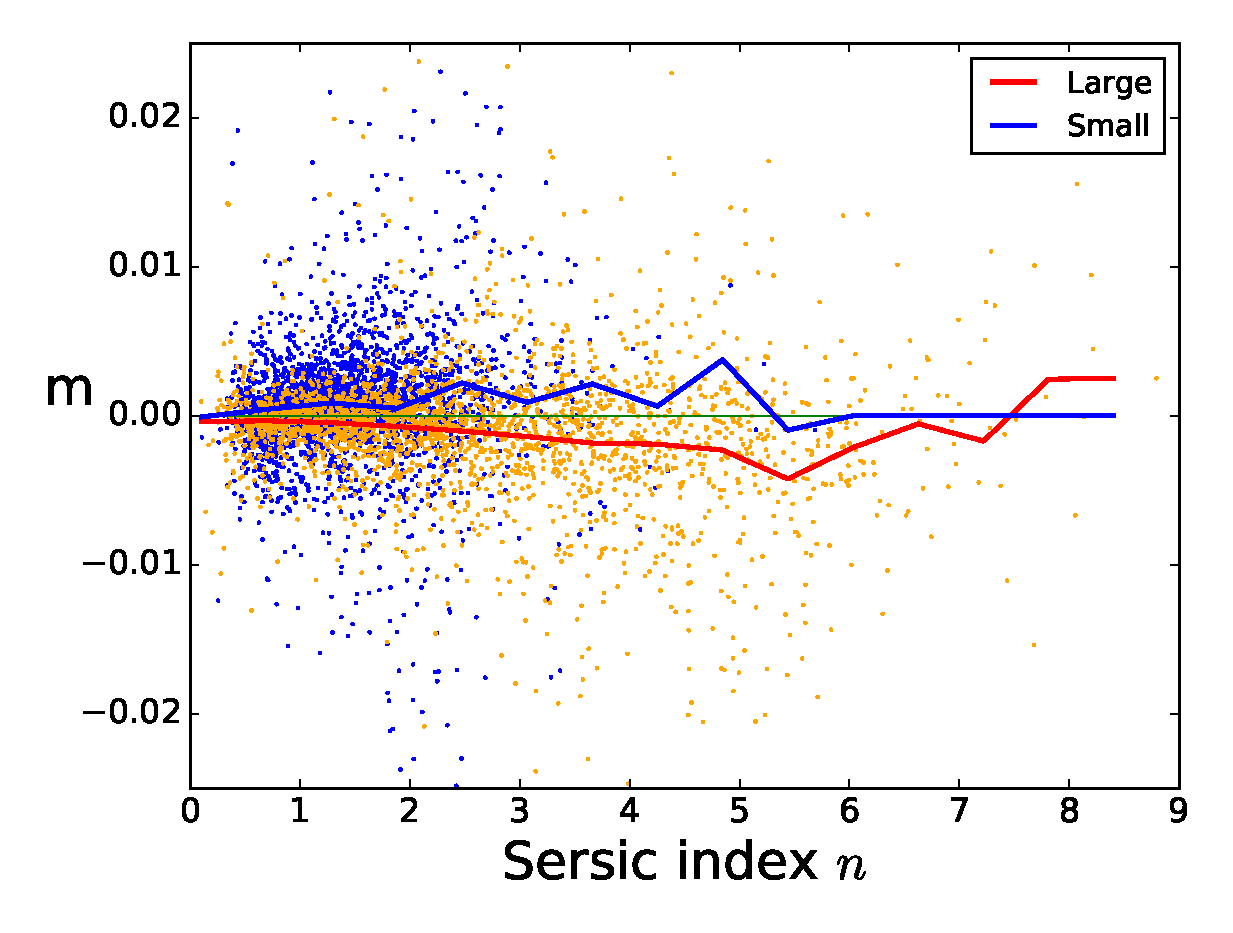
\includegraphics[width=7.0cm]{z2s-ne17.eps}
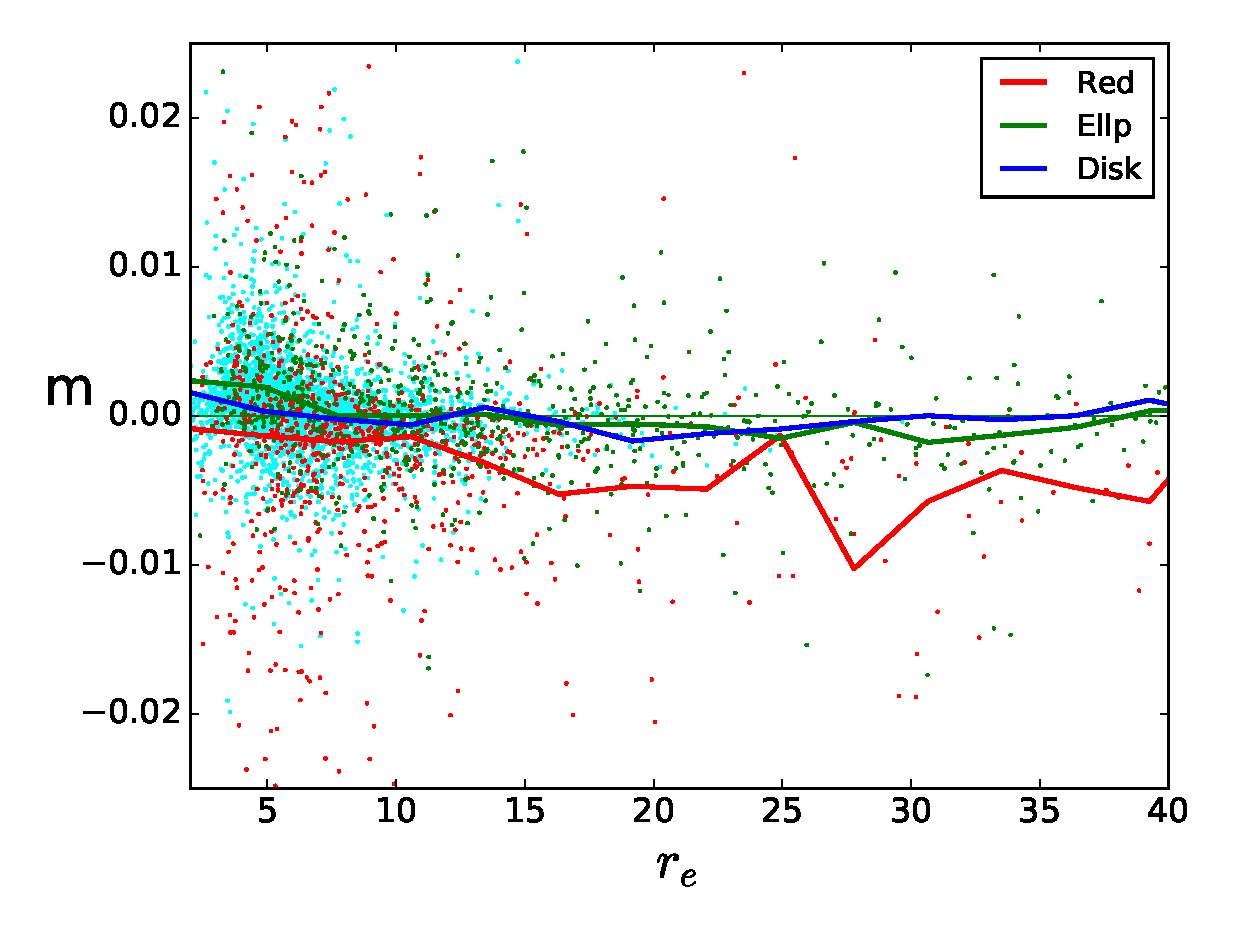
\includegraphics[width=7.0cm]{z2nscl-re17.eps}
\caption{CG bias with Sersic index (top) and effective radius (bottom)
  from the mock VIS images. The unit of radius is a pixel ($=0.05$
  arcsec). In the top panel, the blue (red) is the average of small
  (big) galaxies. In the bottom panel, the red line is average bias of
  red galaxy ($m_{V-I}>1$); the green line is that of elliptical
  galaxy ($n_{Sersic}>2.75$); the blue line is for the disk galaxy.}
\label{fig:cg2re}
\end{figure}
%
The colour gradients as a tracer of galaxy evolution have been found
to be correlate with some aspects. We try to explore relations between
CG bias and the properties of galaxy. First we show the relation
between CG bias with two tracers of the colour gradients: the ratio of
Sersic index from two bands, and the ratio of effective radius from
two bands (Fig. \ref{fig:cg2fitpar}). One can see that there is a
linear relation between the bias and the radius, but for that of
Sersic index it is not obvious. The reason is that the Sersic index is
mainly account for the type of the galaxy, the radius correlates with
the colour gradient directly. Moreover, the CG bias depends on several
factors of the galaxy, e.g. the total size of the galaxy. It is not
surprise to see large bias scatters for the whole sample. In
principle, one expect that when $r_{e606}=r_{e814}$ and
$n_{606}=n_{814}$, the CG bias in principle will be vanish, since the
identical images from two bands will not have a colour gradient. This
is confirmed in our result: the blue line (bin average) in
Fig. \ref{fig:cg2fitpar} meets zero at $r_{e814}/r_{e606}=1$. However,
those colour gradients information will not be available in Euclid. We
also need the relation between the bias with other parameters.


In Fig.\ref{fig:cgbhis}, the galaxies in AEGIS field have more
positive CG bias than the galaxies in the other two. The colour
distribution in AEGIS is different from the other two as well, which
suggests the correlation between the CG bias and the colour of the
galaxy. In Fig.\ref{fig:cg2color}, we show the relation between the CG
bias and the colour of the galaxies. The bias is inversely
proportional to the colour of the galaxies. This is consistent with
the trend of total colour \citep[e.g.][]{2010MNRAS.407..144T}: the
bluer galaxies have positive colour gradients, while the redder ones
have negative gradients. Since this marks a possible transition of two
types of galaxies, we split the galaxy sample into two groups
according to their colour: the red galaxies ($m_{V-I}>0.5$) and the
blue ones ($m_{V-I}<0.5$). They are shown in the bottom panel of
Fig.\ref{fig:cg2color} as a function of redshift. Most of the red
galaxies are located at moderate redshifts, mainly between redshift
$[0.5,1.0]$, while the blue galaxies are either at the lower redshift
($z<0.5$) or higher redshift ($z>1.0$). The CG bias in red galaxies
are obviously more negative than that of the blue ones. It again
confirms that the colour/colour gradients is an important tracer of
the galaxy evolution, since apparently galaxies at different redshift
proceed at different stages of the evolution.

In addition, we stack the images from two bands as our mock VIS band
images, together with the mock VIS magnitude ($m_{VIS}$).  In
Fig.\ref{fig:cg2magvis}, we show the bias as a function of
$m_{VIS}$. There is no obvious dependence on $m_{VIS}$, which seems
conflict with some study of colour gradients,
e.g. \citet{2010MNRAS.407..144T} find tight relation between colour
gradients and $r$-band magnitude. However, there are two points one
needs to notice: 1) the actual $m_{VIS}$ is different from our linear
approximation, also the filter transmission are different of two
telescope. 2) the more important thing is that the wide band magnitude
may not contain sufficient information about the type or colour of
galaxy, thus may not be a good tracer for CG bias.

The VIS image, on the other hand, contains more information
Fig.\ref{fig:cg2re} shows the CG bias with the Sersic index
and the effective radius fitted from the VIS images. In the top panel,
we divide the sample into two groups by the fitted effective radius,
either larger or smaller than $0.35$ arcsec. The small (large)
galaxies are shown by the blue (orange) points, and the blue (red)
line is the bin average.  The large galaxies cover a large range of
Sersic index, have negative average CG bias. Most of small galaxies
have small Sersic index ($<2.5$). The bias of small galaxies are
positive and approximately proportional to the Sersic index. The
scatters of the bias for both large and small galaxies increase with
the Sersic index.
%
In the bottom panel, the galaxies are divide into three groups: the
first is red galaxy whose color is large ($m_{V-I}>1.0$); the second
and third group are the rest galaxies either with large Sersic index
($n>2.25$, elliptical galaxy) or small Sersic index (disk galaxy). The
solid lines show the bin average over effective radius.
%
%\be
%\tilde{m} = a\,r_e+{b\over r_e}+c,
%\elabel{fitcgb}
%\ee
%
%where $r_e$ is the effective radius of the mock VIS image. For disk
%galaxy we have $a=3.8\times10^{-12}$, $b=0.022$, $c=-0.0066$, and for
%elliptical galaxy $a=0.00012$, $b=0.017$ and $c=-0.0069$. The disk
%galaxies have relatively smaller size and smaller CG bias, while the
%elliptical galaxies cover a large range of size and CG bias. Moreover,
%the elliptical galaxies have a stronger dependence on the effective
%radius.
%
We can see that the VIS image alone can also provide an rough
estimation for CG bias, but classification of the galaxies is
necessary. As shown in the figure, the disk galaxies have small bias,
small radius ($<1$ arcsec), and also small bias scatters. The
elliptical galaxies cover large radius range, and the bias is larger
than the disk ones. The bias in red galaxies are significant, and
mainly negative. The scatters of red galaxies are larger than the
other two kinds of galaxies.
%
Extra photometry can definitely provide more constraints on the CG
bias, as it has been shown the correlations between colour gradients and
other properties of galaxy. Moreover, the multi-band
information is required for the photometric redshift study. One can
obtain that for free to calibrate the CG bias. Although the dependence
on the multi-band is different between photometric redshift and CG
bias, the experience from photometric redshift can be used for CG
bias, such as some machine learning algorithms.


We calculate the average bias and the dispersions over the redshift
bins for both red ($m_{V-I}>0.5$) and blue galaxies
(Table\,\ref{table:calibration}). The red galaxies are mainly located
between redshift $(0.4,1.2)$, while the blue galaxies are low density
in redshift $(0.8,1.2)$. The bias from red galaxies are significantly
smaller than that of blue galaxies, as one expected, the colour
gradient in the elliptical galaxies are smaller. The dispersions of
the bias in each bin are large, which probably indicate that in each
bin there are several kinds and sizes of galaxies. Therefore, in
order to calibrate the bias with high precision, one need bigger
galaxy samples. From our simulation, we need about $200$ galaxies for
one type of galaxy in every redshift bin. If we make rough bins, for
instance, 2 types of colour: red and blue; 5 different sizes from
about $0.1$ arcsec to $1.0$ arcsec (Fig.\ref{fig:cg2re}), and 5
redshift bins, at least $20 000$ galaxies are required.  For more
realistic SED classifications and redshift bins, several times larger
sample are also necessary.


\begin{center}
\begin{table}
  \begin{tabular}{llll}
    \hline
    photo-z    &$Number$  &$\bar{m}$  &$\sigma_m$ \\
    \hline
    $0-0.4$   &187  &$-1.3\times10^{-3}$  &$0.012$\\
    $0.4-0.8$  &1415 &$-7.6\times10^{-4}$  &$0.011$\\
    $0.8-1.2$  &1116 &$-1.0\times10^{-3}$  &0.017\\
    $>1.2$  &245  &$-2.1\times10^{-3}$  &0.015\\
    \\
    $0-0.4$  &667  &$6.6\times10^{-4}$  &0.0026\\
    $0.4-0.8$ &513  &$2.8\times10^{-4}$  &0.0028\\
    $0.8-1.2$ &187  &$1.2\times10^{-3}$  &0.0041\\
    $>1.2$  &935  &$5.4\times10^{-4}$  &0.0046\\
    \hline
  \end{tabular}
  \caption{\label{table:calibration}The number, average CG bias and dispersion
  in redshift bins for blue (bottom half) and red (top half) galaxies. }
\end{table}
\end{center}

%\be
%c=m{e_{\rm PSF} \over P_{\gamma}P_{ePSF}},
%\ee
%follow Massey $P_{ePSF}=1$, $P_{\gamma}=0.93$ and using a conservative choice, which corresponds to the maximum value for the polarization allowed for the Euclid PSF $e_{PSF}=0.07$.


\section{Summary and Discussion}
In the image survey for weak gravitational lensing, the wide band
filter can provide high signal-to-noise images and large coverage of
redshift range. There is however a shape bias due to the chromatic
shape of galaxy and the PSF, which is named as colour gradient
bias. For very wide band surveys, such as Euclid, this effect can
cause a non-negligible bias.
%
In this work, we exam such a kind of bias in measuring the shape of a
galaxy using both simulated images and real data taken from the HST
ACS CANDELS survey. In the simulated galaxy images, we confirm the
bias behaviour from previous results (\citetalias{Semboloni13}). We further apply the
calibration method to the noisy images in the simulations, and find
that with reasonable signal-to-noise ratio (SNR$=15$) and sufficient
numbers of galaxies ($300$ images for one type of galaxy in one
redshift bin), we can estimate the CG bias to a high precision.
However, the underestimate cannot be avoided due to strong emission
lines, or the uneven SED of source galaxies. Moreover, the simulations
are performed with only two galaxy models, and the SNR of the
simulated images in two bands are assigned with equal value. In
reality, the relation between the SNR with the size and SED of the
galaxies has to be taken into account.
%
We also perform comparison of TinyTim and star PSF models. The
inaccuracy, especially that due to the binary stars, will cause errors
in estimating the CG bias.


In the estimation using CANDELS data, we select the images from two
filters (F606W, F814W). For most of the galaxy, the bias ($|m|$) is
smaller than $0.01$.  As we find from simulated images, the estimation
using noisy image has a large scatter, thus the CG bias in reality may
be even smaller than that shown here.
%
In our sample of galaxies, the CG bias shows a correlation with the
colour of galaxies, and a linear relation with the ratio of two band
images. We also generate the mock VIS band images. From the parameters
of the image (Sersic index and effective radius), one can classify the
galaxy in order to obtain tighter constraints on the bias. For example,
the galaxies with small Sersic index, i.e. disk-like, have smaller CG
bias. On the other hand, those with large Sersic index have large bias
and also bias variation. The relations show consistent results about
the colour gradient dependence on the properties of galaxy
\citep[e.g.][]{2010MNRAS.407..144T}. However, since the CG bias also
depends on the relative size with respect to the PSF, the dependence
of CG bias is certainly more complicate. We did not provide any
fitting formula for the bias at current sample, since the scatters are
too large. More importantly, it has to be performed according to the
types or morphology of the galaxies, which require larger sample of data.

The multi-band photometry from several bands, which can be used to
estimate the redshift, can be also use for the CG bias analysis.
Although the redshift dependence is not significant in our sample of
galaxies, this may not be the case for a larger survey, or if we look
at the bias according to the type of galaxy. Moreover, the colour of
galaxy also indicates the evolution history, or the large scale tide
force.  It can be also used for the study of intrinsic alignment
analysis in weak lensing \citep[e.g.][]{2015SSRv..193....1J}.
Therefore, the dependence of the CG bias on the colour of the galaxies
will further increase the sysmatics of the intrinsic alignment. The
detail behaviour will require large cosmological simulations, which is
beyond the scope of this paper, but definitely needs further studies for
the project such as Euclid.

The role of environment on the colour gradients is not clear. On the
one hand, it has been shown that colour gradients depend on the
environment where galaxies reside, with steeper colour gradients in
poor rather than rich clusters \citep[e.g.][]{2005ApJ...626L..19L},
which is possible due to the different processes during galaxy
formation. On the other hand, in recent study using integral field
spectra from SDSS-IV, the metallicity gradients show weak or no
correlation with density environment \citep{2017MNRAS.465.4572Z}. In
any cases, close galaxy pairs or nearby bright star(s) may also cause
weak brightness/colour gradient, which will affect our estimate for CG
bias as well. 

In this work, we use the brightness moments to estimate the
ellipticity of the galaxy. The PSF correction is not taken into
account. The bias thus will appear in every method of measurement.
However, the bias using the measurement method for real data
will be different, since every method has its own property and weight
function. The CG bias will have method-dependent properties as well,
although they will in principle have same dependence on the colour
gradient of the galaxy images. As the first step of the CG bias
analysis, we did not adopt any specific method in order to obtain
general properties of the CG bias. Before the real analysis of Euclid
data, one needs to study the bias with specific methods and simulated
images with real properties in the Euclid weak lensing survey.

%
%Moreover, as we point out that higher order image distortions, such as
%flexion may increase the CG bias. It can be seen from our analysis
%using both simulated and CANDELS data. Although the higher order
%effect can be neglected most times, it can still significantly
%increase the CG bias when the source images are located close to the
%strong lensing region. Therefore, such a kind of effect may cause
%significant bias in the strong lensing analysis using wide band
%images. In galaxy-galaxy lensing and cluster lensing, one needs to
%be careful about such higher order effects as well.

\section*{Acknowledgments}

We would like to thank Emiliano Merlin, Marco Castellano for helping
on SExctractor and Galfit, Gary Berstein, Adam Rogers and
also in general, the members of the Euclid Consortium for useful
discussions.  XE and VFC are funded by Italian Space Agency (ASI)
through contract Euclid -IC (I/031/10/0) and acknowledge financial
contribution from the agreement ASI/INAF/I/023/12/0. XE is also partly
support by NSFC Grant No. 11473032. JR is supported by JPL, which is
run by Caltech under a contract for NASA, and is supported by grant
NASA ROSES 12-EUCLID12- 0004. The fast Fourier transforms are supplied
by the FFTW library \citep{fftw05}. We use CFITSIO
\citep{1999ASPC..172..487P} for the FITS file.

\bibliographystyle{aa}
\bibliography{cbias}

\end{document}
